\documentclass[12pt]{report}
\usepackage[german]{babel}
\usepackage[utf8]{inputenc}
\usepackage{fontspec}
\usepackage{fancyhdr}
\usepackage{mathrsfs}
\usepackage{amssymb}
\usepackage{amsmath}
\usepackage{amsfonts}
\usepackage{float}
\usepackage{caption}
\usepackage{tikz}
\usepackage{tikz-uml}
\usetikzlibrary{automata,arrows,positioning,shapes}
\tikzstyle{activity} = [rectangle, draw, text centered, text width=7em, rounded corners, minimum height=2em]
\tikzstyle{dia} = [diamond, draw]
\tikzstyle{invis} = []
\usepackage{textcomp}
\usepackage{verbatim}
\usepackage{booktabs, tabularx}
\usepackage{graphicx}
\usepackage{multicol}
\usepackage{paralist}
\usepackage{enumitem}
\usepackage{acronym}
\renewcommand\tabularxcolumn[1]{m{#1}}
\setlist[itemize,1]{label=$\bullet$}
\setlist[itemize,2]{label=$\bullet$}

\pagenumbering{arabic}
\pagestyle{fancy}
\rhead{Analyse von Projektlastenheften}
\renewcommand{\footrulewidth}{1pt}
\renewcommand{\arraystretch}{0.6}

\begin{document}
\begin{titlepage}
\raggedright
\begin{large}
Entwurf und Implementierung einer Werkzeugunterstützung zur sprachlichen Analyse und automatisierten Transformation von Projektlastenheften im Kontext der Automobilindustrie
\end{large}

\vfill\vfill\vfill\vfill
An der Fachhochschule Dortmund\\
\vfill
im Fachbereich Informatik\\
\vfill
Studiengang Informatik\\
\vfill
Vertiefung Praktische Informatik\\
\vfill
erstellte Thesis\\
\vfill\vfill\vfill\vfill
zur Erlangung des akademischen Grades\\
\vfill
Bachelor of Science\\
\vfill
B. Sc.\\
\vfill\vfill\vfill\vfill
von Aaron Schul, \\
\vfill
geboren am 24.06.1997\\
\vfill
und Felix Ritter\\
\vfill
geboren am 31.08.1997\\
\vfill\vfill
Betreuung durch:\\
\vfill
Prof. Dr. Sebastian Bab und Prof. Dr. Steffen Helke\\
\vfill
Dortmund, 28.02.2019\\
\end{titlepage}

\newpage
\begin{abstract}
Ein weitläufiges Problem in der Autoindustrie ist die effiziente Verarbeitung von Pflichtenheften. Einer der Gründe dafür ist, dass viele verschiedene Bereiche bei der Entwicklung der Fahrzeuge und sogar kleinster Einzelteile beteiligt sind. So müssen zu Beginn einer Produktentwicklung etwa Betriebswirtschaftler, Designer, Techniker und Ingenieure zusammen ein Dokument entwerfen, das die Produktmerkmale widerspiegelt. Darin müssen die Anforderungen an das gewünschte Produkt so genau beschrieben sein, sodass es anhand dieses Dokuments entwickelt werden kann. Als Experten ihrer jeweiligen Domäne weiß dabei jeder genau, was dazu nötig ist. Sobald jedoch Auswirkungen über die eigene Domäne hinausgehen, kann es schnell passieren, dass Widersprüche oder Abhängigkeiten entstehen. Diese werden später schnell übersehen, da solche Zuständigkeiten nicht eindeutig geklärt sind. Das Resultat ist dann ein Fehler in der Entwicklung, welcher von zeitlicher Verzögerung über zusätzliche Kosten bis hin zum Abbruch des Projekts führen kann. 
Methoden aus dem Natural Language Processing (NLP) können dabei helfen, die Überprüfung der Pflichtenhefte auf Konsistenz stark zu vereinfachen oder sogar teilweise zu automatisieren. Dafür kann beispielsweise der Text in den Lastenheften analysiert und dessen Inhalt innerhalb einer Wissensbasis, sog. Ontologie, abgespeichert werden.
In dieser Arbeit wird daher die Entwicklung zweier NLP-basierter Werkzeuge zur Vereinfachung bzw. Lösung dieser Probleme vorgestellt werden. Zum einen ein \textit{Requirements-to-Boilerplate-Converter}-Werkzeug (R2BC), welches dem Nutzer helfen soll, das Pflichtenheft eines Auftraggebers in die betriebsinternen Richtlinien und Standards zu überführen. Zum anderen wird der \textit{Delta-Analyser} vorgestellt, welcher auf dem R2BC aufbaut, indem er automatisch zwei homogene Lastenheft vergleicht und dadurch im Kontext des gesamten Pflichtenhefts Widersprüche und Abhängigkeiten herausstellt. 
Ziel ist es dabei, jeweils einen Prototypen als \glqq\textit{proof of concept}\grqq, also als Machbarkeitsstudie, zu implementieren. Nach dieser Vorstellung wird zusätzlich das weitere Potential der Programme erläutert, welches sich bei der Entwicklung der Prototypen gezeigt hat. Diese bietet Vorschläge zur weiteren bzw. vollständigen Implementierung der Programme.

\end{abstract}

\renewcommand{\abstractname}{Abstract}
\begin{abstract}
A widespread problem in the auto industry is the efficient processing of specifications. One of the reasons for this is that many different areas are involved in the development of vehicles and even the smallest of parts. For example, at the beginning of product development, managers, designers, technicians, and engineers all need to design a single document together. The requirements for the desired product must be described in such detail that it can be developed using this document. As experts in their domain, everyone knows exactly what is needed. However, as soon as effects go beyond the own domain, it can quickly happen that contradictions or dependencies arise. These are quickly overlooked later, as such responsibilities are not clearly clarified. The result is then a mistake in the development, which can lead from time delay over additional costs up to the demolition of the project.
Methods from Natural Language Processing (NLP) can help to simplify or even partially automate the review of functional specifications for consistency. For example, the text in the specifications can be analyzed and its contents stored within a knowledge base, so-called ontology.
In this work, therefore, the development of two NLP-based tools to simplify or solve these problems will be presented. On the one hand, there is a program called Requirements-to-Boilerplate Converter (R2BC), which should help the user to transfer the specifications of a client into the company's internal guidelines and standards. On the other hand, the so-called delta analyzer is shown, which is based on the R2BC, in that it automatically compares two homogeneous specification sheets and thereby highlights contradictions and dependencies in the context of the entire specification.
The goal here is to implement a prototype as a proof of concept of the program concepts from ZIC19. Due to the limited resources of this work, a list with further potential of the programs, which has been shown during the development of the prototypes, is additionally explained. This offers suggestions for further or complete implementation of the programs.
\end{abstract}

\newpage
\tableofcontents
\newpage
\listoffigures
\listoftables
\newpage

\thispagestyle{empty}
\begin{huge}
Abkürzungsverzeichnis
\end{huge}
\vspace{12pt}
\begin{acronym}[Abkürzungsverzeichnis]
\acro{CRS}{Customer Requirement Specification}
\acro{DA}{Delta-Analyser}
\acro{E-AE}{Electronics-Advanced Engineering}
\acro{NLP}{Natural Language-Processing}
\acro{OEM}{Original Equipment Manufacturer}
\acro{OWL}{Web-Ontology-Language}
\acro{PMT}{Projects, Methods and Tools}
\acro{POS}{Part-Of-Speech}
\acro{R2BC}{Requirements-To-Boilerplate-Converter}
\acro{RE}{Requirements-Engineering}
\end{acronym}
\newpage

\thispagestyle{empty}
\textbf{Danksagung}
\vspace{12pt} \\
An dieser Stelle möchten wir uns bei allen Personen bedanken, die uns bei unserer Bachlorarbeit und während des Studiums begleitet und unterstützt haben.
\vspace{12pt} \\
Der Dank gebührt unseren Familien und Freunden aus der Heimat und aus dem Studium für ihre Unterstützung.
\vspace{12pt} \\
Wir danken auch allen Kollegen aus der Abteilung E-AE bei der Firma HELLA in Lippstadt für ihr Interesse und die großartige Zusammenarbeit. Die einzigartigen Erfahrungen, die wir während unseres Praktikums und später während der Bachelorarbeit in der Firma sammeln konnten, haben uns wirklich motiviert. Besonderer Dank geht dabei an Konstantin Zichler, der weit mehr als nur Betreuer in der Firma, sondern auch Mentor und Ideengeber unserer Arbeit war.
\vspace{12pt} \\
Schlussendlich danken wir unseren Betreuern Prof. Dr. Sebastian Bab und Prof. Dr. Steffen Helke für die zahlreichen Tipps und Anregungen während der Bachelorarbeit.
\newpage

\newpage
\chapter{Einführung}
\section[Motivation]{Motivation und thematische Grundlagen}
In einer Vielzahl von Firmen stellt die Erhebung von Anforderungen den ersten Schritt bei der Entwicklung von neuen Produkten dar. Diese Anforderungen manifestieren sich später in der zu entwickelnden Hard- und Software. Spätere Produktmerkmale müssen dabei weit vor der tatsächlichen Entwicklung berücksichtigt werden und fließen in das Anforderungsdokument ein. Die Erhebung und Identifikation dieser Anforderungen wird als \textit{Requirements-Engineering} bezeichnet \cite{bal10}.

Dieser Prozess wird dabei sowohl bei kompletten Neuentwicklungen, als auch bei der Adaption eines bereits vorhandenen Produktes auf neue Projekte durchlaufen. Zur Rolle von Requirements-Engineering in Projekten siehe etwa \cite{mw02} und \cite{hl01}. 

Dem Betrieb liegen anschließend die Aufgaben und Ziele für die Entwicklung als Dokumente vor, auf deren Basis die Produktentwicklung beginnen kann. Die Entwicklung unterliegt dabei bestimmten Kriterien und Faktoren, die den unternehmerischen Erfolg beeinflussen. Neben betriebswirtschaftlichen Einflüssen wie der Einordnung des Produktes in der Wertschöpfungskette sind es dabei besonders technische Anforderungen an das Produkt, die definiert und während der Produktentwicklung eingehalten werden müssen.

\subsubsection{Anforderungen im betrieblichen Entwicklungsprozess}
Das Resultat ist das sogenannte Pflichtenheft, in Unternehmen häufig als CRS (\textit{Customer Requirement Specification}) bezeichnet \cite{dge19}. Mithilfe dessen kann nun die Entwicklung eines Produktes begonnen werden. Ein später hergestelltes Produkt sollte möglichst allen beschriebenen Anforderungen entsprechen. Da Betriebe jedoch nur selten alle einzelnen Komponenten des späteren Produktes selbst herstellen können, sind sie auf Zulieferer angewiesen, die einzelne Komponenten entwickeln und produzieren. Diese Hersteller einzelner Komponenten werden als \textit{OEM} (\textit{Original Equipment Manufacturer}), zu Deutsch \textit{Erstausrüster}, bezeichnet \cite{ir09}.  

In diesem Fall wird dem Zulieferer ein Pflichtenheft übergeben, dass allen Anforderungen des Kunden genügt. Das bedeutet jedoch, dass auch die Produktentwicklung anhand des Pflichtenheftes an den Zulieferer ausgelagert wird. Dem Zulieferer werden damit Möglichkeiten geboten und Verantwortung übertragen, das Produkt weiter zu definieren. Einerseits können etwa interne Richtlinien und Erfahrungen auf dem Gebiet der Produktentwicklung aus früheren Projekten integriert werden, andererseits aber auch weitere Optimierungen sowie Merkmale, die noch nicht im Pflichtenheft dokumentiert sind. Somit agiert der Zulieferer nicht nur als produzierende Fabrik, sondern nimmt am Entwicklungsprozess teil.

Die Anforderungen an ein Produkt, etwa technische Rahmenbedingungen und Qualitätsanforderungen, setzen sich dabei aus einer Auflistung von funktionalen und nicht-funktionalen Anforderungen zusammen \cite{bal10}. Häufig enthält das Pflichtenheft auch weitere Informationen und abseits von Text Abbildungen, die einzelne Anforderungen ergänzen. 

\subsubsection{Umstände der Anforderungsdefinition}
Die Anforderungen werden dabei von vielen verschiedenen Domänenexperten beim OEM formuliert und in das Pflichtenheft für die Entwicklung eingetragen. Verschiedenste Akteure aus einem Unternehmen sind dabei an der Festlegung der Anforderungen an ein Entwicklungsprojekt bzw. Produkt beteiligt. Beteiligte sind etwa Produktdesigner, Ingenieure und Systemtechniker, die an verschiedenen Stellen im Lastenheft Anforderungen an eine Komponente festlegen und an entsprechenden Stellen vermerken. Diese Beteiligten sind in der Regel auf ihren Bereich spezialisiert und nicht interdisziplinär, da häufig an verschiedenen Orten und an spezifischen Aspekten eines Produktes in mehreren Projektteams entwickelt wird. 

Projektteams aus einem Bereich tauschen sich häufig nicht untereinander aus und legen unabhängig von anderen Beteiligten Anforderungen fest. Demzufolge sammeln sich im Lastenheft schon bei der Entstehung beim OEM verschiedenste Merkmale einer Komponente, die aber nicht im Bezug zueinander stehen und sich im schlimmsten Fall gegenseitig ausschließen. Ferner gibt es sprachliche Eigenheiten der Autoren und sprachliche Fehler, die innerhalb des Teams nicht auffallen und später nicht mehr korrigiert werden. Auch gibt es unternehmensinterne Richtlinien für die Formulierung von Anforderungen beim OEM, die das Verständnis auf Seite des Zulieferers erschweren können. Christian Allmann, Lydia Winkler und Thorsten Kölzow haben in \cite{awk06} solche Herausforderungen für das Requirements-Engineering zwischen OEMs und Zulieferern identifiziert.

Durch die entstehende große fachliche Breite und Tiefe der Spezifikationen im Pflichtenheft, können mitunter Dokumente mit einem Umfang von von mehreren tausend Seiten entstehen. Dies bedeutet einen hohen Aufwand bei der Transformation und Bündelung der Anforderungen in ein tatsächliches Produkt beim Zulieferer. 

\subsubsection{Prozessoptimierung durch Werkzeuge}
Bei der Untersuchung von Projektlastenheften muss also nach Zusammenhängen und Bezügen zwischen mehreren Anforderungen gesucht werden, damit die Korrektheit des späteren Produktes gewährleistet ist. Die Analyse von Zusammenhängen zwischen Anforderungen stellt dabei aus Gründen der Effizienz ein Problem dar, wenn jeder Projektbeteiligte von Hand die für ihn relevanten Anforderungen aus dem Lastenheft extrahieren muss. Auch müssen die Lastenhefte an die Formulierungen und Ausdrucksweisen für Requirements-Management im Unternehmen angepasst werden. 

Bislang gibt es jedoch kaum Werkzeugunterstützung, die effiziente Möglichkeiten zur automatisierten Überarbeitung und Anpassung einzelner Anforderungen aus dem Dokument bietet. Ansätze aus dem \textit{Natural-Language-Proessing}, kurz NLP, stellen gleichzeitig vielversprechende Forschungsfelder in der Informatik dar, die eine solche automatisierte Verarbeitung auf Basis von Sprachanalyse ermöglichen. Diese werden in Kap. 2 ausführlich erläutert. Syntax und Semantik der einzelnen Sätze und Zusammenhänge in Texten können auf Basis aktueller Trends wie Machine-Learning und dynamischer Programmierung zunehmend besser abgebildet werden.

\section[Unternehmenskontext]{Unternehmenskontext der Arbeit}
Besonders betroffen von dem geteilten Entwicklungsprozess zwischen OEMs und Zulieferern ist die Automobilindustrie. Eine Vielzahl von Zulieferern beliefert die Automobilhersteller mit Komponenten für ihre Fahrzeuge. Einzelne Komponenten bestehen dabei häufig auch aus mehreren Einzelteilen, die wiederum von mehreren verschiedenen Zulieferern geliefert werden. \cite{awk06}

\subsection{Einsatz bei HELLA}
Einer dieser Zulieferer ist die HELLA GmbH \& Co. KGaA (im folgenden (die) HELLA genannt), die sich auf die Entwicklung und Produktion von Licht- und Elektronikkomponenten in Hard- und Software spezialisiert hat. HELLA ist ein international operierender deutscher Automobilzulieferer mit Hauptsitz in Lippstadt und zählt zu den Top 100 Automobilzulieferern weltweit \cite{lv10}. Für weitere Information siehe \cite{he19} sowie die Firmenwebsite. 

Zum Verfassen dieser Arbeit waren die Autoren fünf Monate bei der Firma beschäftigt. Dies beinhaltete zwei Monate Arbeit als Praktikanten und die verbleibenden drei Monate als Bacheloranden. 
Die Hauptaufgabe dort war die Mitarbeit im Bereich Requirements-Engineering für die Abteilung der Elektronik-Vorentwicklung \textit{E-AE} (\textit{Electronics-Advances Engineering}). 

Die Abteilung ist zuständig für die Planung und Umsetzung von Vorentwicklungsprojekten um die Ergebnisse an die Serienentwicklung oder verschiedene OEMs weiterzuleiten. Dies beinhaltet häufig, wie zuvor beschrieben, den Austausch von Informationen der Firma HELLA mit diversen OEMs bezüglich gemeinsamer Projekte. Die genaue Darstellung dieser Prozesse erfolgt in Kap. 3.1. Somit erhält diese Abteilung auch oft Lastenhefte der OEMs, welche dann an die Projektteams weitergeleitet werden. 

\subsection{Anforderungsmanagement im Unternehmen}
Die Gewichtung einzelner Anforderungen in einem größeren Systemkontext fällt dort schwer, da nun Projektteams beim Zulieferer, die an der Entstehung des Lastenheftes nicht beteiligt waren, dieses verstehen sollen und auf ihre Teilkomponente anwenden müssen. Zusätzlich zu den teilweise widersprüchlichen Anforderungen aus dem Pflichtenheft kommen weitere Anforderungen des Zulieferers, wie etwa die Gewinnmarge und unternehmensinternte Richtlinien hinzu. Schlussendlich soll jedoch ein Produkt entwickelt werden, dass möglichst alle Anforderungen berücksichtigt. \cite{mw02}

Zu diesem Zweck können bei Zulieferern spezielle Abteilungen existieren, die Projektteams bei der Identifikation und Gewichtung von Anforderungen unterstützen. Diese Abteilungen sind auf die Auswertung der Projektlastenhefte spezialisiert und erstellen Modelle zu Merkmalen des späteren Produktes. Die Experten stellen dabei die Eindeutigkeit und Verständlichkeit sicher und identifizieren relevante Anforderungen für die Mitglieder des Projektteams. Somit kann ein eigenes Anforderungsdokument für das Projektteam beim Zulieferer erstellt werden. 
Falls nicht vorhanden, muss das Team selbst über die Bewertung von Anforderungen entscheiden und Rücksprache mit dem OEM halten.

Bei HELLA existiert eine dementsprechende Abteilung, genannt \textit{Projects, Methods and Tools}, kurz \textit{PMT}. Im Rahmen unserer Beschäftigung konnte in enger Zusammenarbeit mit PMT genau ermittelt werden, wie Lastenhefte momentan verarbeitet werden, welche Verbesserungspotentiale dabei bestehen und wie diese genutzt werden können.

\section{Hypothese}
Hypothese dieser Arbeit ist, dass sich mithilfe von NLP Lastenhefte effizient automatisiert verarbeiten lassen. Damit kann die Arbeit von Requirements-Engineers, aber auch von Beteiligten an der Entwicklung beim Verständnis der Anforderungen, erleichtert werden. Dabei ist die Auswertung der Syntax und Semantik für ein tieferes Verständnis von Textzusammenhängen, also von verschiedenen Anforderungen, relevant.

Die sprachliche Analyse kann Requirements erkennen und kategorisieren, sowie in Beziehung zueinander setzen. Insbesondere lassen sich die beschriebenen Probleme bei der Überprüfung der Pflichtenhefte auf Konsistenz lösen oder zumindest vereinfachen. Dies kann mithilfe der in dieser Arbeit beschriebenen Programme geschehen, welche konzeptuell dargestellt und prototypisch implementiert werden. 

Weiterhin soll geprüft werden, wie stark ein Mehrwert bei der Nutzung solcher Programme für ein Firma ausfallen kann. Dies beinhaltet ersparte Arbeitszeit, Kosten und vermiedene Fehler. 

\section{Methodik}
Verschiednene Methoden aus dem Bereich Natural Language-Processing werden zunächst anhand des Rückblicks auf die Projektarbeit theoretisch und anhand praktischer Beispiele erläutert. Der betriebliche Kontext der Firma HELLA wird durch genaue Darstellung der dortigen Verfahren beleuchtet. 

Mit diesen Grundlagen wird dann die Unterstützung der dortigen Prozesse im Bereich Requirements-Engineering auf Basis von natürlichsprachlicher Textanalyse evaluiert. Die gewonnenen Erkenntnisse aus der Zusammenarbeit mit der Abteilung PMT wurden in Anforderungen an die zu entwickelnden Werkzeuge zusammengefasst, die als Basis für unsere Softwareentwicklung dienten. Dadurch entstand eine genaue Vorstellung der zu entwickelnden Software, welche mit Hilfe der Programmkonzepte von Konstantin Zichler ZIC19 entworfen und implementiert werden konnte. 

Das Ergebnis stellten zwei Software-Prototypen auf \textit{java}-Basis dar, deren Struktur und Funktionsweisen wir anhand von Modellen und Codebeispielen darstellen. Die Prototypen wurden mit originalen Pflichtenheften von verschiedenen OEMs und der HELLA getestet und evaluiert.

\section{Aufbau der Arbeit}
In der folgenden Ausarbeitung wird zunächst in Kapitel 2 eine Überblick über den Stand der Technik gegeben. Dies beinhaltet einerseits einen Rückblick auf die zuvor verfasste Projektarbeit zu NLP und einer Erläuterung der Grundlagen von Ontologien und andererseits einen Überblick von Arbeiten, die sich der gleichen oder ähnlichen Problemstellungen gewidmet haben. 

Kapitel 3 beschäftigt sich für eine bessere Einordnung der beiden Programme mit dem betrieblichen Umfeld bei der HELLA. Hierzu wird zunächst, vor dem Hintergrund des momentanen Vorgehens, der Anwendungsfall der Programme genauer beschrieben. Somit lassen sich die betrieblichen Anforderungen an die Werkzeuge bestimmen, welche dann von den vorgestellten Konzepten abgedeckt werden sollen. 

In Kapitel 4 wird das erste Werkzeug - der R2B-Converter - ausführlich beschrieben. Dies beinhaltet die Darstellung dessen Architektur, eine Vorstellung der Implementierung, eine Auflistung möglicher Erweiterungen und eine genaue Beschreibung des Testverfahrens der Software. Zu den Tests werden dabei präzise die Methodik, die Durchführung und die Ergebnisse vorgestellt, welche in dem späteren Evaluations-Kapitel aufgegriffen und eingeordnet werden. 

Das zweite Werkzeug - der Delta-Analyser - wird in Kapitel 5 behandelt. Dabei werden ähnlich zu Kapitel 4 die Architektur, die Implementierung, mögliche Erweiterungen und durchgeführte Tests beschrieben. Es wird genau dargelegt wie die Testergebnisse erzielt wurden, die später zusammen mit den Ergebnissen von Kapitel 4 evaluiert werden, um das Resultat der beiden Werkzeuge bewerten zu können. 

Kapitel 6 stellt das zuvor erwähnte Evaluations-Kapitel dar. Hier findet zunächst die Auswertung der erhobenen Testergebnisse statt.
Anschließend wird anhand dessen dargestellt, ob und inwiefern das Nutzen der Werkzeuge einen Mehrwert für die Firma erwirtschaften kann und somit im betrieblichen Umfeld eingesetzt werden sollte.  
Somit lässt sich die Korrektheit der in 1.2 gestellten Hypothese überprüfen.

Die Arbeit wird von Kapitel 7 abgeschlossen. Dieses beinhaltet eine Zusammenfassung der geleisteten Arbeit und der Ergebnisse. Außerdem wird zuletzt noch ein Ausblick für die Zukunft der Werkzeuge und die Lösung des Problems erläutert. 

\section{Autorenverzeichnis}
\begin{multicols}{2}
\begin{compactitem}
\item[] \textbf{1.: Ritter, Schul}

\begin{compactitem}
\item[] 1.1: Ritter
\item[] 1.2: Ritter
\item[] 1.3: Ritter, Schul
\item[] 1.4: Schul
\item[] 1.5: Schul
\end{compactitem}

\item[] \textbf{2.: Ritter, Schul}
\begin{compactitem}
\item[] 2.1: Schul
\end{compactitem}

\end{compactitem}
\end{multicols}

\chapter{Stand der Technik}
In diesem Kapitel wird zunächst ein Rückblick auf die zuvor von den Autoren verfasste Projektarbeit und die darin enthaltenen Grundlagen von NLP gegeben. 
Aufgrund ihrer besonderen Relevanz für die Programme werden anschließend zusätzliche Ontologien als Teil von NLP genauer beleuchtet. 
Außerdem wird mit Hilfe von verwandten Arbeiten ein Überblick über die Problematik und verschiedene Lösungsansätze geboten. 

\section[Rückblick auf die PA]{Rückblick auf die Projektarbeit}
In \cite{rs18} sind die Grundlagen von NLP im Rahmen einer Projektarbeit zusammengefasst. In diesem Abschnitt werden die für die Arbeit relevanten Aspekte kurz wiederholt. 
\subsection{Grundlagen zu Natural Language Processing}
\subsubsection{Definition und Ziel}
Natural Language Processing ist zu verstehen als die automatisierte oder halb-automatisierte Verarbeitung von natürlicher Sprache mit Hilfe eines Computers. In NLP sind verschiedenste wissenschaftliche Bereiche verknüpft.\footnote{Es ist anzumerken, dass verschieden weit gefasste Definitionen von NLP existieren. Manche schließen etwa auch die Erfassung von Sprache mit ein, etwa durch Interaktion mit Sprachcomputern. Andere beschränken sich ausschließlich auf den Verarbeitungsprozess der Sprachdaten im Computer selbst, siehe 2.1.2.} Hauptsächlich handelt es sich dabei um Linguistik und Informatik, jedoch gibt es auch viele Verbindungen zur Psychologie, Philosophie Mathematik und Logik. \cite{cop04}

Ziel von NLP ist üblicherweise die Extraktion von Informationen aus einem Text durch kleinschrittige Textanalyse. Diese Informationen werden dem Text direkt über sogenannte Annotationen angehängt oder anders abgespeichert, etwa in Ontologien, welche in einem späteren Abschnitt genauer erläutert werden.

\subsubsection{Beispiele von Forschung und Entwicklung}
Die wissenschaftliche Erforschung von NLP entstand Mitte des 20. Jahrhunderts, als der Linguist Noam Chomsky zeigte, dass sich Merkmale der englischen Sprache formalisieren und somit automatisieren lassen \cite{cho57}. 

Frühe Projekte wie der Sprachcomputer ELIZA aus den 1960er Jahren waren somit bereits in der Lage eine natürlichsprachliche Frage als Texteingabe entgegenzunehmen und üblicherweise eine plausible Antwort zu liefern.   

Heutzutage gibt es ein Vielzahl von Spracherkennungssoftware auf Smartphones oder Smart-Devices wie ALEXA, welche in der Lage sind gesprochene Kommandos zu erkennen und über das Internet an Server zu leiten, welche in der Lage sind diese Kommandos schnell und effizient zu verarbeiten \cite{hao14}.

\subsubsection{Herausforderungen von NLP}
Durch die Verbindung von Linguistik und Informatik stellt sich NLP generell der Herausforderung sowohl inhärente Probleme der Sprache, als auch Probleme der Automatisierung lösen zu müssen. 

Zu den sprachlichen Problemen gehören Aspekte wie Mehrdeutigkeit, Sarkasmus und Umgangssprache bzw. Redewendungen. Diese lassen sich oft nicht einzig und allein durch den gegebenen Text erklären, sondern beruhen auf Kontext und Situation.

Vor allem bei der Erfassung von Semantik, also dem Inhalt der Texte, können komplexe Probleme auftreten. So gibt es beispielsweise Mehrdeutigkeiten, welche selbst für den Menschen nicht einfach zuzuordnen sind. So kann \glqq \textit{Die Betrachtung des Studenten}\grqq etwa bedeuten, dass der Student etwas betrachtet. Genauso kann es jedoch sein, dass jemand anderes den Studenten betrachtet. 

Eine andere häufige Fehlerquelle ist das korrekte Zuordnen von sprachlichen Bezügen. Betrachtet man die Frage \glqq \textit{Verkaufen Sie Handys und Computer von Samsung}\grqq, so ist diese eindeutig grammatikalisch korrekt. Dennoch ist es uneindeutig, ob sich die Frage auf nach der Marke der Handys richtet, oder ob dies lediglich auf die Computer bezogen ist. 

Noch komplexer wird es, wenn sich diese Bezüge über verschieden Sätze bzw. Teilsätze erstrecken. So ist der Satz \glqq \textit{Tom schenkt Tim ein Fahrrad, weil er nett ist}\grqq ebenfalls auf zwei verschieden Arten zu deuten. Einerseits kann es sein, das Tom das Fahrrad verschenkt, weil Tom ein netter Mensch ist, andererseits kann es sein, das Tom das Fahrrad verschenkt, weil Tim nett zu ihm ist. 

Weiterhin können auch bei der korrekten Erfassung des Sprachinhalts weitere Probleme die Kommunikation stark beeinflussen. So kann etwa die Intention der Sprache dem Inhalt widersprechen, wie es bei Sarkasmus üblicherweise der Fall ist. 

Bei der Implementierung ergeben sich dann Probleme, trotz der sprachlichen Besonderheiten konsistente Regelmäßigkeiten als Grundlage zur Automatisierung zu finden. 

\subsubsection{Linguistische Analyse}
Um einen Text möglichst Fehlerfrei verarbeiten zu können bedarf es also einem kleinschrittigen und präzisen Verfahren. Dieses bezeichnet man als linguistische Analyse.

Sie ist aufgeteilt in vier wichtige Schritte, welche aufeinander aufbauen und an Komplexität zunehmen. Im folgenden sind diese Schritte aufgeführt und kurz erläutert \cite{rs18}:

\begin{enumerate}
\item
Morphologische Analyse - Die Zerlegung von Wörtern bezüglich ihrer Struktur. Die Komposition aus Präfix, Wortstamm und Suffix von Wörtern wird erkannt, um Fall, Tempus, Numerus etc. des Wortes zu bestimmen. Im Englischen zeigt so die Endung -ed bei Verben die Vergangenheitsform an. Dabei ist zu beachten, dass Mehrdeutigkeiten entstehen können.
\item
Syntax - Aufbau von Sätzen durch einzelne Wörter. Jede Sprache besitzt syntaktische Regelungen bezüglich der auftauchenden Wörter; im Deutschen folgt etwa auf einen Artikel irgendwann ein Substantiv oder bestimmte Signalwörter geben Satztyp und Tempus an. Auf Basis dieses Wissens können formale und strukturelle Analysen der Textbestandteile erfolgen.
\item
Semantiken - Die Identifikation der Bedeutung von einzelnen Sätzen und Wörtern. Die Semantik eines Textabschnittes wird häufig als \glqq  Logik\grqq{} bezeichnet und fragt nach dessen Bedeutung bzw. Thema. Semantische Deutungen können anhand von Kompositionen einzelner Wörter und Sätze auf Basis der semantischen Analyse erkannt werden.
\item
Kontext - Darstellung von satzübergreifenden Zusammenhängen syntaktischer und semantischer Natur. Mehrere Sätze können über Konstrukte wie etwa Pronomen verbunden sein, wenn sich das Pronomen des einen Satzes auf ein Subjekt des anderen bezieht. 
\end{enumerate}

Diese Aufteilung lässt sich jedoch in noch weitere Teilschritte für die Spracherkennung und -generierung als NLP-Architektur unterteilen. Diese wird im folgenden Abschnitt genauer erläutert. 

\subsection{Umsetzung der Verarbeitungsschritte natürlicher Sprache}
Dieser Abschnitt beschäftigt sich primär mit den verschiedenen Schritten der sprachlichen Analyse. Diese Differenzierung kann dabei, wie zuvor beschrieben, anhand der linguistischen Analyse unterschiedlicher Bestandteile von Sprache vorgenommen werden. Diese sukzessive Verarbeitung wird im folgenden anhand verschiedener Algorithmen und Verfahren erläutert, die im wesentlichen in \cite{rs18} zu finden sind. 

Das Ziel jeder Analyse ist es, Wissen über einen Teilbereich von Sprache zu generieren. Das Wissen über den Zusammenhang von Wörtern eines Textes kann eindeutig sein, jedoch können besonders bei der morphologischen Analyse sprachliche Mehrdeutigkeiten auftreten. Dies wird in 2.1.3-Morphologie näher erläutert. 

Die Präzision dieser Aussagen fällt dementsprechend abhängig von der Treffergenauigkeit und dem Abdeckungsgrad der linguistischen Analyse durch die verwendeten Verfahren ab. Es ist dabei zu beachten, dass die Analyse typischerweise als Architektur aufgebaut ist, da die verschiedenen Schritte aufeinander aufbauen \cite{cop04}. Somit können, basierend auf den Ergebnissen, inhaltliche Aussagen und Zusammenhänge über den zugrundeliegenden Text getroffen werden. 

\cite{cop04} identifiziert dabei eine allgemeine NLP-Architektur, die basierend auf der linguistischen Analyse diese Teilbereiche voneinander abgrenzt. 
Für ein besseres Verständnis der Verfahren werden die für diese Arbeit relevanten Schritte in \cite{rs18} wie folgt kurz erläutert:

\begin{enumerate}
\item
Input Processing - Erkennung der Dokumentensprache und Normalisierung des Textes. Im ersten Schritt geht es um das korrekte Format des Eingabedokumentes für die Verarbeitung. Dieser Vorgang stellt jedoch noch keine Analyse dar, sondern dient lediglich der Vorbereitung.
\item
Morphologische Analyse - Die meisten Sprachen sind im Bezug auf ihre Grammatik und syntaktische Struktur der Wörter in Systemen abgeschlossen, etwa durch Modellierung mittels Automaten zur Erzeugung der Worte. Auch können Vokabeln in Wörterbüchern/Lexika gesammelt und Regeln auf ihnen formuliert und gespeichert werden.
\item
Part-of-Speech-Tagging - Die einzelnen Wörter eines Satzes werden im Hinblick auf den Sach- oder Satzzusammenhang, wie auch auf die Stellung im Satz hin analysiert. Basierend auf Kontext und/oder Erfahrungswerten bzw. Heuristiken können die Wörter korrekt erfasst und deren Fall getaggt werden. Subjekte, Prädikate usw. werden identifiziert. Dazu kann eine Wissensbasis mit Trainingsdaten und die Einordnung des Kontextes darin verwendet werden.
\item
Parsing - Die Ergebnisse der vorherigen Schritte werden weiter verarbeitet und in ein standardisiertes Format gebracht. Syntaktische Zusammenhänge, wie etwa das Zusammenfassen von Wörtern zu einer gemeinsamen Bedeutungsphrase und das Zuordnen von Verben zu einem Nomen können nach dem Parsing dargestellt werden.
\item
Disambiguation - Die Entfernung von Mehrdeutigkeiten auf Basis der Ergebnisse des Parsings stellt einen entscheidenden Schritt für die semantischen Analysen dar. Nur wenn die Aussage und der Kontext eines Satzes klar erkennbar sind, kann dessen Semantik gezielt abgeleitet werden.
\item
Context Module - Textbausteine, deren Interpretation semantisch auf dem Kontext anderer Sätze oder Wörtern beruhen, können erfasst werden. Bei Anaphern ist etwa das Verständnis des aktuellen Kontexts abhängig von einer vorherigen Deutung.
\item
Text Planning - Die Sachzusammenhänge und Semantiken, die aus dem zugrundeliegenden Text extrahiert wurden, werden für die Darstellung im fertigen Text definiert. Es wird festgelegt, welche der Bedeutungen qualitativ übertragen und vermittelt werden sollen. Die Reihenfolge und Umfang der behandelten Themen wird geschätzt und definiert.
\item
Tactical Generation - Die Bedeutungen werden in Form konkreter Zeichenketten generiert, die die gewünschte Bedeutung enthalten. Diese Textbausteine basieren häufig direkt auf den Ergebnissen des vorherigen Parsings, da dort schon Bedeutungen zusammengefasst werden können. Der quantitative Teil des Textes wird erzeugt.
\item
Morpholigical Generation - Die erzeugten Sätze werden morphologisch an die Rahmenbedingungen der verwendeten Sprache angepasst. Grammatiken und Regeln der Satzkonstruktion werden auf die erzeugten Wörter angewendet, sodass ein lesbarer und nachvollziehbarer Text entsteht.
\item
Output Processing - Der Text wird nun, nachdem dieser inhaltlich komplett erzeugt vorliegt, an das Design und Format des jeweiligen Einsatzzwecks angepasst. Sollte Text, anders als in dieser Arbeit der Einfachheit halber angenommen, nicht als geschriebenes Wort ohne besondere Formatierung vorliegen, kann dieser einem \textit{Formatter} zur Designanpassung übergeben werden. Ferner kann etwa mihilfe von Text-to-Speech eine Audioausgabe erfolgen. 
\end{enumerate}

Wie später gezeigt wird, kann die in dieser Arbeit beschriebene Entwicklung der Software-Prototypen als eine Umsetzung eben dieser NLP-Architektur verstanden werden.

\subsection[Syntaktische Analyse]{Syntaktische Analyse von Wörtern und Sätzen}
In diesem Abschnitt wird die Zerlegung der Syntax anhand logischer Modelle von Sprache beschrieben. Begonnen wird mit der einfachen Struktur und Zusammensetzung einzelner Wörter aus der Grammatik. Die Kombination aus Wortstämmen mit Prä- und Suffixen kann etwa in einem Lexikon gesucht werden, dass alle Wörter einer Sprache enthält.  Basierend auf dieser Morphologie eines Wortes kann dann in der Analyse mehrerer Wörter auf die Rolle von Wörtern im Satzzusammenhang geschlossen werden. 

\subsubsection{Morphologie}
Dieser Abschnitt befasst sich genauer mit der Analyse der Struktur und Zusammensetzung von Wörtern. Dies wird als morphologische Analyse bezeichnet. Wie im folgenden beschrieben, können auf dieser Basis logische Modelle wie etwa Automaten erstellt werden, die zulässige Wörter aus einer Sprache auf Basis grammatikalischer Regeln erzeugen können. Für ein besseres Verständnis der im Rahmen dieser Arbeit vorgestellten Ergebnisse beschränkt sich diese Arbeit auf die vergleichsweise einfach strukturierte englische Sprache. Aufgrund der großen Fortschritte und Erfahrungen in der Sprachforschung, werden die folgenden Beispiele auf Englisch behandelt.

In der englischen Sprache besteht jedes Wort aus einem Wortstamm, sowie den sogenannten Affixen. In einem Satz könnte etwa das Wort \glqq \textit{believable} \grqq auftauchen. Das Wort stammt von der Grundform \glqq \textit{(to) believe} \grqq (zu Deutsch: \glqq glauben \grqq) ab. Das \textit{-able} stellt ein Suffix dar, also eine Wortendung. Zusammen mit den Präfixen, die dem Wortstamm vorangestellt sind, gehört \textit{-able} somit zur Kategorie der Affixe. 

Das Ziel der morphologischen Analyse ist nun, die Zusammensetzung des Wortes nachzuvollziehen und die Information für die weitere Verarbeitung bereitzustellen. Die Generierung des Wortes \textit{believable} kann anhand von Buchstabierregeln erfolgen, die alle zulässigen Wörter auf englisch anhand der Wortstämme und Affixe erzeugen können. Es fällt auf, dass in unserem Beispiel \textit{believable} vor dem Hinzufügen des Suffixes \textit{-able} zunächst das \textit{-e} von der Grundform \textit{(to) believe} entfernt werden muss. Eine Grammatik, die zur Erzeugung dieser Wörter genutzt werden kann, muss dementsprechend eine solche Regel vorhanden sein. Gemäß \cite{rs18} bedeutet dies formal ausgedrückt:
\tt
\begin{center}
e $\rightarrow \varepsilon \textasciicircum \_$able
\end{center}
\rm

In der Logik kann man diese Regeln als nicht-deterministischer \textit{Zustandswandler} visualisieren.\footnote{In \cite{rs18} wurde darauf hingewiesen, dass nicht-deterministische Zusatandswandler trotzdem mithilfe der \textit{Potenzmengenkonstruktion} in einen äquivalenten deterministischen Zustandswandler überführt werden kann. Sie kommen somit zu einem eindeutigen Ergebnis \textit{erzeugbar} oder \textit{nicht erzeugbar} in der Sprache.} In Abb. 2.1 ist der Zustandswandler gezeigt, die das Suffix \textit{-able} an entsprechende Wörter anhängen kann.
\\

\begin{figure}[h!]
\begin{center}
\begin{tikzpicture}
\node[accepting] (a) at (0,0)  [circle, draw, minimum size=10ex] {1};
\node (b) at (4,0)  [circle, draw, minimum size=10ex] {2};
\node (c) at (4,-4) [circle, draw, minimum size=10ex] {3};
\node[accepting] (d) at (0,-4) [circle, draw, minimum size=10ex] {4};
\draw[thick, ->] (a) to [bend left] node[midway, above] {$\varepsilon$ : e} (b);
\draw[thick, ->] (a) to [loop above] node[midway, above] {other : other} (a);
%\draw[thick, ->] (b) to [bend left] node[midway, below] {e : $\varepsilon$} (a);
\draw[thick, ->] (b) to [bend left] node[midway, right] {$\varepsilon : \textasciicircum$} (c);
\draw[thick, ->] (c) to [bend left] node[midway, below] {able:able} (d);
\end{tikzpicture}
\caption{Nicht-deterministischer Zustandswandler der able-Regel \cite{rs18}}
\end{center}
\end{figure}
Um alle zulässigen Wörter sammeln und identifizieren zu können, muss die morphologische Analyse über eine Menge an Informationen über die Sprache verfügen.
Die Bestandteile von Wörtern können dabei in verschiedenen Lexika enthalten sein, welche die entsprechenden Informationen bereitstellen. Gemäß \cite{cop04} bedarf es dabei drei verschiedener Lexika:

\begin{enumerate}
\item Liste von \textit{Affixen} (zusammen mit den Informationen, die damit verbunden sind, z.B. Negation \tt \glqq  un-\grqq{}\rm)
\item Liste von \textit{unregelmäßigen Wörtern} (zusammen mit den Informationen, die damit verbunden sind, z.B. \tt \glqq  went\grqq{}:simple past\glqq  (to) go\grqq{}\rm)
\item Liste von \textit{Wortstämmen} (zusammen mit syntaktischer Kategorie, z.B. \tt \glqq  believe\grqq{}:verb\rm)
\end{enumerate}

Es ist zu beachten, dass die in der morphologischen Analyse verwendeten Buchstabierregeln zwar zu jeweils eindeutigen Ergebnissen kommen können, die Analyse selbst jedoch nicht eindeutig sein muss. Dies kann, wie bereits zuvor beschreiben, durch sprachliche Mehrdeutigkeiten entstehen. 

Das Wort \glqq \textit{even}\grqq könnte isoliert etwa einmal als \textit{gleichmäßig}, also als Adjektiv kategorisiert, ins Deutsche übersetzt werden, jedoch auch sinngemäß \textit{sogar}, also das Adverb mit einem oder mehreren Bezugswörtern meinen.\footnote{Aus Gründen der Vereinfachung wurde sich hier auf zwei erkennbar verschiedene Bedeutungen beschränkt. Tatsächlich stellt sich neben Bestimmung des grammatikalischen Typs auch die Frage, ob sich die verschiedenen Übersetzungen derselben Kategorie, z.B. \textit{even} als \textit{gerade} und \textit{gleichmäßig}, in ihrer Bedeutung im Sachzusammenhang unterscheiden.} Die mehreren möglichen Bedeutungen des einzelnen Wortes können jedoch in der Regel durch die Position und grammatikalische Funktion im Satz aufgelöst werden. Diese Eigenschaften werden durch das \textit{Part-of-Speech-Tagging} identifiziert.

\subsubsection{Part-Of-Speech-Tagging}
Die Ergebnisse der morphologischen Analyse von mehreren Wörtern, etwa in einem Satz, können zur Analyse von Zusammenhängen zwischen diesen Wörtern genutzt werden. Somit kann die grammatikalische Struktur des Satzes auf Basis der einzelnen Wörter dargestellt werden. Der grammatikalische Typ jedes Wortes wird durch das Part-Of-Speech-Tagging festgelegt und jedes Wort wird \textit{annotiert}. Wie später in dieser Arbeit beschrieben wird, dienen solche Annotationen in NLP-Werkzeugen der Sammlung der bekannten Informationen zu einem Wort oder Satz. 

Zur Festlegung dieser grammatikalischen Funktionen werden sog. \textit{POS-Tagger} eingesetzt, die verschiedene Worttypen als Kategorien beinhalten. Diese werden dann jedem Wort eines Satzes als Annotation hinzugefügt. Die Aufgabe ist es nun, die korrekte Funktion eines Wortes im Satz auf Basis der morphologischen Analyse zu identifizieren. 

Als Beispiel soll der Satz 
\\
\tt
\\I love trains.\\
\\ \rm 
dienen. Das Part-of-Speech tagging zum Wort \glqq \textit{trains}\grqq soll hier veranscheulicht werden. Das Wort \glqq \textit{trains}\grqq allein ist ein Nomen im Plural, jedoch könnte es sowohl das Subjekt, als auch das Objekt im Satz darstellen. im Im Englischen sollte ein POS-Tagger aber erkennen, dass \textit{Subjekt-Prädikat-Objekt} eine gültige Satzkonstruktion darstellt, die zu dem Beispielsatz passt. Dementsprechend entfällt die Möglichkeit von \textit{trains} als Subjekt, da es hinter einem Verb als Akkusativobjekt des Satzes auftaucht.

Es existieren verschiedene Techniken für diese Beurteilungen der POS-Tagger. Verschiedene gültige Satzkonstruktionen sind häufig als sog. \textit{corpora} gespeichert. Diese stellen repräsentative Trainingsdaten dar, die beispielsweise aus der Zeitung \textit{Wall-Street-Journal} stammen. 
In diesem Corpus könnten etwa die annotierten Sätze
\\
\tt
\\People(subj) love(vb) trains(obj) .(punc)
\rm und\\
\tt
I(subj) go(vb) home(obj) .(punc)\\
\\ \rm
enthalten sein.\footnote{Die tatsächliche Annotation kann durch POS-Tagger i.d.R. feiner erfolgen, sodass etwa Pronomen von Subjekten unterschieden werden. Auch können, wie später in dieser Arbeit gezeigt wird, eigene Annotationen bei Bedarf nach neuen Kategorien hinzugefügt werden. Der Corpus hier stellt ein stark vereinfachtes Beispiel dar. Ein ausführliches Beispiel unter der Verwendung der CLAWS-7-POS-Taggers findet sich in \cite{rs18}.}

Mithilfe dieser Menge von Daten kann POS-Tagging auch heuristisch, d.h. auf Basis von Wahrscheinlichkeiten bzw. Metriken, erfolgen, indem das Auftauchen verschiedener Satzbauten im Trainingscorpus gezählt wird. Auf dieser Basis können dann Wahrscheinlichkeiten für verschiedene Möglichkeiten berechnet werden, wenn es mehrere mögliche Zuordnungen gibt. 

\subsubsection{Nutzen syntaktischer Analyse für NLP}
Ein wichtiges Einsatzgebiet für POS-Tagger ist auch die Wortvorhersage bzw. \textit{prediction} auf Basis solcher Heuristiken. Diese kann im Kontext der zuvor vorgenommen Annotationen von Wörtern erfolgen. Beispielsweise werden sog. \textit{n-gramme} verwendet, um unter Berücksichtigung der Annotation von \textit{n} gelesenen Wörtern die Möglichkeiten für das folgende Wort zu berechnen. In \cite{rs18} findet sich ein vollständiges Beispiel anhand eines \textit{Bigramms} mit Corpus.

Die heutigen Verfahren zur syntaktischen Analyse nutzen zur Steigerung der Genauigkeit u.a. Verfahren aus dem maschinellen und automatisierten Lernen und können somit hohe Trefferquoten erzielen.\footnote{In \cite{she07} wird ein POS-Tagger auf der Basis von bidirektionaler Analyse und Machine-Learning zum Erstellen der Trainingsdaten beschrieben. Obwohl nur auf Basis der Textsyntax erzielt, sind die Ergebnisse zu 97,33\% korrekt.} Um ein tieferes Verständnis von Texten zu erzielen, reicht die in diesem Abschnitt beschriebene syntaktische Analyse anhand der Grammatik nicht aus. Die tatsächliche Abbildung von Wissen über semantische Zusammenhänge stellt eine verlässlichere Möglichkeit dar, sprachliche Zusammenhänge zu identifizieren. 

\subsection{Umgang mit Semantik}
Wie im letzten Abschnitt aufgezeigt wurde, können nicht alle Informationen aus einem Text eindeutig anhand der Erfassung der Grammatik eines Satzes extrahiert werden. Die Syntax eines Satzes ist häufig mehrdeutig, da der Zusammenhang einzelner Wörter verschieden interpretiert werden kann. Auf der semantischen Ebene, d.h. der Bedeutung, existieren jedoch bereits bei einzelnen Wörtern verschiedene Deutungen. 

Schon bei der Mensch-Mensch-Kommunikation kommt es somit häufig zu Missverständnisse, wenn die Bedeutung hinter einer Aussage nicht eindeutig ist. Auf Basis des Kontextes einer Aussage bzw. der Domäne des Inhalts kann jedoch meist zu einer mehrdeutigen Aussage eine eindeutige Deutung identifiziert werden.

NLP beschäftigt sich daher auch intensiv mit der Abbildung und Modellierung der Semantik von Sprache, die in der Logik häufig als \glqq \textit{Logik einer Aussage}\grqq bezeichnet wird.\footnote{Bereits in den 1980er Jahren wurden Konzepte auf Basis logischer Modelle, mit denen Semantik abgebildet werden kann, mithilfe von Theorembeweisern und Model-Checking beschrieben. \cite{sb88} \cite{kn85}} Die Formalisierung mehrerer Bedeutungen kann dabei mithilfe von Symbolen der Aussagenlogik erfolgen, die Symbole dienen dabei als Platzhalter für Wörter bzw. Satzteile. Etwa das Beispiel aus \cite{rs18}:

\tt
Every man loves a woman.
\rm
\\
Zu deutsch \textit{\glqq  Jeder Mann liebt...\grqq{}} ist semantisch mehrdeutig zwischen  
\begin{enumerate}
\item \textit{\glqq  ...die eine Frau\grqq{}}: $\exists y [woman'(y) \bigwedge \forall x [man'(x) \Rightarrow love'(x,y)]]$ und
\item \textit{\glqq  ...irgendeine Frau\grqq{}}: $\forall x [man'(x) \Rightarrow \exists y [woman'(y) \bigwedge love'(x,y)]]$
\end{enumerate}

Bereits durch den Menschen fällt die Deutung anhand von Symbolen der Aussagenlogik nicht leicht. Daher wurden verschiedene Arten von Zusammenhängen, u.a. auf Basis von Symbolen der Mengenlehre, anhand welcher die Deutung vereinfacht und klarer erkennbar wird. 

\subsubsection{Meaning-Postulates}
Linguisten und Philosophen haben Regeln für die Abbildung von Zusammenhängen auf eindeutige Kategorien formalisiert. Dabei wurden verschiedene Bedeutungen von Wortzussammenhängen identifiziert, die als (Bedeutungs-)Mengenbeziehung bzw. Relation zwischen Symbolen visualisiert werden können \cite{car52}:

\begin{enumerate}
\item \textit{Meaning-Postulates}: A beinhaltet B und C

Der Begriff A setzt sich logisch aus der Relation zwischen B und C zusammen, etwa:

$\forall x[bachelor(x)\Rightarrow man(x)\bigwedge unmarried(x)]$

sinngemäß:\glqq \textit{Ein Junggeselle ist ein Mann und nicht verheiratet}.\grqq

\item \textit{Hyponomy}: A ist ein B

\tt
Ein Hund ist ein Tier. 
\rm

Also hat ein Hund auch alle Eigenschaften eines Tieres. Auf Basis solchen Wissens kann eine Kategorisierung erfolgen bzw. lassen sich verscheidene Ausprägungen der gleichen Sache zusammengefassen \cite{rs18}.

\item \textit{Meronymy}: A $\subseteq$ B, A ist Teil von B

\item \textit{Synonymy}: A $\equiv$ B, A ist semantisch äquivalent zu B

\item \textit{Antonymy}: A $\equiv \neg$B, A bedeutet das Gegenteil von B
\end{enumerate}

Feinheiten der Deutung, wie etwa der Unterschied von \glqq \textit{A semantisch äquivalent zu B}\grqq{} zu \glqq \textit{A ist ein B}\grqq{} müssen dabei während der Erstellung semantischer Modelle unterschieden werden, da die Kategorisierung sonst zu grob ausfällt. Es können sonst falsche Zusammenhänge und Beziehungen entstehen, die Fehlinterpretationen der Aussagen erzeugen.

In der Praxis stellt sich daher die Frage, in welchem Umfang Semantiken für NLP tatsächlich für eine Verbesserung der Textanalyse sorgen und wie detailliert eine Modellierung dazu erfolgen muss. Mit diesem Ansatz beschäftigen sich die \textit{Ontologien} in Kapitel 2.2.

\subsubsection{}

\section{Ontologien}

Dieser Abschnitt befasst sich genauer mit dem Begriff der Ontologien im Kontext der Informatik. 

\subsection{Definition}
Ontologien lassen sich allgemein definieren als \glqq formale, schematische Abbildungen eines Wissensbereichs, bestehend aus einem Vokabular und Regeln zu seiner Zusammensetzung\grqq \cite{we13}.

Zunächst bedeutet dies, dass eine Ontologie stets auf nur Wissen aus einer bestimmten Domäne bezieht und nicht versucht das gesamte über die Welt bzw. sehr allgemeines Wissen abzubilden. 

Des weiteren Besteht eine Unterteilung in ein Vokabular und in eine Menge von Regeln. 

Einer der Aspekte von Ontologien, welche sie für die Informatik so geeignet machen ist, dass sie in maschienenlesbaren Ontologiesprachen verfasst werden. Somit können Computersysteme diese automatisch auslesen und ggf. interpretieren und daraus schlussfolgern. 

Da Terminologie und bestimmte Formalitäten zwischen Ontologiesprachen variieren können, wird im Folgenden der Bezug auf die weit verbreitete Ontologiesprache \glqq Web Ontology Language\grqq{} (OWL) angenommen.

\subsection{Aufbau}
Der Aufbau von Ontologien lässt sich grob in zwei Aspekte unterteilen: 

\begin{enumerate}
\item Das Vokabular: Hier sind alle Dinge innerhalb des Wissensbereiches aufgeführt, welcher von der Ontologie abgedeckt werden soll. Dazu gehören sowohl die Oberbegriffe dieser Dinge, als auch die Instanzen selbst. 
\item Die Regeln: Diese beschreiben die Dinge genauer und bilden deren Beziehung untereinander ab. Sie können eigenständig existieren oder im Bezug zu den vorhandenen Dingen stehen. 
\end{enumerate}
\subsubsection{Klassenhierarchie}
Die Hierarchie einer Ontologie, also der strukturelle Aufbau, lässt sich in die folgenden drei Komponenten unterteilen:
\begin{enumerate}
\item Begriffe: Die Grundlage für die Struktur einer Ontologie stellt der hierarchische Aufbau von \textit{Begriffen} (\textit{concepts}). Diese Repräsentieren eine Art Klassenstruktur und werden daher oft auch als Klassen bezeichnet. Sie können in aus der Informatik bekannten Ansätzen wie Ober- und Unterklassen angeordnet werden. Begriffe sind üblicherweise sehr generell gehalten und könnten etwa die Klasse \textit{Auto} abbilden. 

\item Typen: In vielen Fällen lässt sich ein Begriff in verschiedene \textit{Typen} aufteilen. Ein Auto kann beispielsweise nach verschiedenen Automarken typisiert werden. Diese Typen werden dann ebenfalls durch Klassen verkörpert und bilden in dem hierarchischen Aufbau eine Unterklasse des jeweiligen Begriffs. Da sowohl Begriffe, als auch Typen in Klassen verkörpert werden, wird in der Praxis oftmals nicht zwischen den beiden unterschieden. Man kann jedoch üblicherweise über einer Unterklasse als Typ der Oberklasse sprechen. 

\item Instanzen: Die sogenannten \textit{Instanzen} (\textit{instances}) verkörpern konkrete Objekte dieser Klassen und werden nicht weiter aufgespalten bzw. typisiert. Ein Instanz wäre dann etwa ein bestimmtes Modell, einer bestimmten Marke von Autos. 
\end{enumerate}

Diese Hierarchie ist ggf. beliebig erweiterbar. So könnte man für eine bessere Klassifizierung z.B. die Marke eines Autos zunächst in eine Produktreihe oder nach einer Produkteigenschaft wie \textit{Combi} typisieren und erst davon abhängig die verschiedenen Instanzen zuordnen.

In Abbildung X.X ist eine stark vereinfachte Klassenhierarchie aus Oberklassen, Unterklassen und Instanzen beispielhaft dargestellt. 
\\
\newline
HIER KLASSENHIERARCHIEBILD EINFÜGEN
\\
\newline
Auf der obersten Ebene der Klassen-Hierarchie befindet sich die Klasse \textit{owl: Thing}. Von dieser erben alle Begriffe durch die \textit{hasSubclass}-Relation. Dies ist vergleichbar mit der objektorientierten Programmiersprache \textit{Java} bei welcher alle Klassen direkt oder indirekt von der Oberklasse \textit{Object} erben. 

Auf der nächsten Ebene befinden sich die beiden Begriffe \textit{Automobil} und \textit{Person}. Diese können entweder direkt in Instanzen übergehen, oder zunächst durch Typisierung unterteilt werden. 

Somit finden sich in der nächsten Ebene die drei nach Marke getrennten Automobil-Typen \textit{VW}, \textit{BMW} und \textit{Audi}. Außerdem werden Autofahrer und Ingenieure als Personen unterschieden. Es ist anzumerken, dass es nicht ausgeschlossen ist, das ein Ingenieur auch Autofahren ist. Wegen der möglichen Mehrfachvererbung lassen sich jedoch Typen oder Instanzen erzeugen, welche sowohl von Autofahrer, als auch von Ingenieur erben. Somit stellt eine Unterteilung in Typen ohne gegenseitigen Ausschluss in der Praxis kein Problem dar und kann sogar nützlich sein, wie später anhand von Relationen gezeigt wird. 

In der vierten Ebene sind einzig zu Demonstrationszwecken einige der Typen weiter unterteilt und andere nicht. Man sieht, dass die Hierarchie also keineswegs gleichmäßig sein muss, um eine sinnvolle Unterteilung zu gewährleisten. 

In der letzten Ebene befinden sich einige Instanzen von Autos welche durch konkrete Modelle dargestellt werden. Theoretisch ließen sich auch diese weiter unterteilen, etwa nach Innenausstattung. Diesbezüglich ist je nach Verwendungszweck der Ontologie genau festzulegen, wie die Hierarchie zu strukturieren und wie weit sie auszuführen ist. Beispielsweise macht es für einen großen Autohersteller keinen Sinn, wenn in einer konzernübergreifenden Ontologie jeder Ingenieur instantiiert ist.

\subsubsection{Regeln}
Die Regeln in einer Ontologie lassen sich in die folgenden zwei Komponenten unterteilen:
\begin{enumerate}
\item Relationen: Einen wichtigen Bestandteil von Ontologien bilden die sogenannten \textit{Relationen} (\textit{properties}).
Relationen beschreiben Beziehungen zwischen Begriffen und werden oft auch als Eigenschaften verwendet und bezeichnet. Ähnlich zu vielen Programmiersprachen können diese Relationen und Eigenschaften eines Begriffs an die Instanzen des Begriffs vererbt werden. Grundsätzlich ist dabei auch eine Mehrfachvererbung möglich. 

\item Axiome: Des Weiteren können Ontologien durch sogenannte \textit{Axiome} (\textit{restictions})  genauer modelliert bzw. eingeschränkt werden. Axiome verkörpern dabei Regeln in der Ontologie welche stets zutreffen müssen. Üblicherweise werden diese dazu verwendet, Einschränkungen vorzunehmen, die nicht effizient durch den abgebildeten Wissensbereich darzustellen sind. Dies könnte Beispielsweise in einer Ontologie über verschiedene Automodelle verschiedenster Marken eine generelle Definition von Automobilen sein. 
So ließe sich die Voraussetzung, dass ein Automobil motorisiert sein muss durch eine Klasse \textit{Bauteil} mit der Unterklasse \textit{Motor} darstellen, welche dann über eine \textit{muss verbaut sein in}-Relation mit der Klasse \textit{Automobil} verbunden ist. Ist es jedoch nicht Zweck der Ontologie Bauteile genauer abzudecken, wäre dies unnötiger Aufwand, der außerdem die Übersichtlichkeit der Ontologie einschränken könnte.
\end{enumerate}

Abbildung X.X zeigt eine beispielhafte, stark vereinfacht Ontologie zu Automobilen und bestimmten im Kontext relevanten Personen. 
\\
\newline
HIER RELATIONEN BILD
\\
\newline
Die Relationen zwischen den Konten der Ontologie sind dargestellt durch Linien mit einem mittigen Pfeil. Die durchgezogenen Linien zeigen den Grundaufbau der Hierarchie. Die blauen Linien verkörpern die \textit{has subclass}-Beziehung, welche auf Vererbung hinweist. Die violetten Linien stehen für die \textit{has individual}-Beziehung und zeigen auf eine Instanz der Klasse. 
Außerdem wurden zwei Objekt-Attribute (\textit{object properties}) manuell hinzugefügt. Diese können verwendet werden um Relationen zwischen Klassen aufzuzeigen, welche nicht voneinander erben, sondern sich in unterschiedlichen \glqq Teilbäumen\grqq{} der Ontologie befinden. So verweist, dargestellt durch den braunen Pfeil eine \textit{benutzt}-Relation von dem Autofahrer auf das Automobil, bedeutet also das Autofahrer Automobile verwenden.  
Ähnlich dazu zeigt von der Klasse Ingenieur eine \textit{entwickelt}-Beziehung auf Automobil.
\\
\newline
NACHSCHAUEN WEGEN VERERBUNG AUF INSTANZEN.
\subsubsection{Verwendung von Ontologien}
Wie eingehend bereits erwähnt sind Ontologien vor allem in der Informatik durch ihre Maschinenlesbarkeit wertvoll. Sie sind außerdem auch geeignet komplexere Sachzusammenhänge abzubilden, was mit primitiven Datentypen wie man sie in einer relationalen Datenbank abspeichern kann nicht möglich wäre. Simple Verbindungen wie sie etwa in den in 2.1.4 beschriebenen Bedeutungspostulaten beschrieben sind lassen sind in Ontologien schnell und effizient darstellen.

Betrachte man zum Beispiel das Satzschema \glqq B ist ein A\grqq{} so würde dies durch eine einfache \textit{hasSubclass}-Beziehung von der Klasse \textit{A} zu der Klasse \textit{B} dargestellt.
Erstellt man nun die beiden Instanzen \textit{b1} und \textit{b2} der Klasse B, so liegen implizit bereits die Informationen vor, dass sie beide auch ein \textit{A} sind. Außerdem ist ihre Homogenität durch die Abstammung von der gleichen Klasse gewährleistet. Daher brauchen die Instanzen hierfür weder eine Beziehung untereinander, noch zu der Oberklasse \textit{A} ihrer Elternklasse \textit{B}.
\\
\newline
Grafik mit A,B,b1 und b2 und Tier, Vierbeiner, Hund und Katze
\\
\newline

Im Zusammenhang dieser Arbeit sollen später Ontologien dazu verwendet werden den Inhalt betrieblichen Anforderungen aus einem Pflichtenheft abzuspeichern. Pflichtenhefte sind dabei stark domänenbezogen und somit optimal geeignet um in Ontologien abgespeichert zu werden. Des Weiteren lassen sich stets Relationen zwischen den einzelnen Teilbereichen ziehen, was für einen einzelnen Domänenexperten schwierig wäre. Eine üblicherweise vorausgesetzte Eigenschaft für Anforderungen ist Atomarität [QUELLE], was bedeutet, dass jeder Satz nur genau eine Aussage beinhalten soll. Dies hat zur Folge, dass viele betriebliche Anforderungen tatsächlich den vorgestellten, knappen Satzschemata entsprechen.

\section{Verwandte Arbeiten}
Dieses Kapitel stellt einen Überblick über bereits veröffentlichte Arbeiten dar, die sich mit dem Themen Natural Language Processing für Anforderungsmanagement, sowie die Unterstützung durch Werkzeuge beim Requirements-Engineering befassen. 

\subsubsection{Grundlage dieser Arbeit}
K. Zichler und S. Helke stellen in \cite{zh17} und \cite{zh19} die wesentlichen Aspekte für den Entwurf einer Softwareunterstützung für Requirements-Engineering in Firmen vor. 

In \cite{zh17} wird zunächst der Bedarf nach solcher Unterstützung besonders für die Automobilindustrie beschrieben, da die Verbesserung herkömmlicher Methoden im Requirements-Engineering dort wesentliches Potential bietet. Der Vorschlag beinhaltet die Unterstützung von Projektteams durch ein Expertenteam aus Requirements-Experten, die Anforderungen aufbereiten und deren konsistente Umsetzung verbessern. 

Auf dieser Basis stellen sie in \cite{zh19} konkret einen Entwurf eines Werkzeugs für die automatisierte Analyse von Projektlastenheften vor. Das Werkzeug gliedert sich dabei in eine Komponente zur Überführung natürlichsprachlicher Anforderungen in vordefinierte Sprachschablonen, genannt Requirements-to-Boilerplate-Converter (\textit{R2BC}). Auf dieser Basis arbeitet dann der \textit{Delta-Analyser} der die Unterschiede zwischen mehreren Lastenheften, die in Schablonen überführt sind, darstellen kann. Dabei kommen auch Ontologien und NLP-Methoden zum Einsatz. Die Prototypen basieren dabei auf der Open-Source-Software \textit{GATE} zur sprachlichen Auswertung und sollen als 3-Schichten-Architektur umgesetzt werden. 

Diese Arbeiten stellen die wesentliche Grundlage für die in unserer Arbeit entworfenen Prototypen dar. Die Implementierung erfolgte in Zusammenarbeit mit dem Autoren Konstantin Zichler bei der Firma HELLA, die den konkreten Anwendungsfall für seine Entwürfe und unsere Umsetzung dargestelt hat.

\vspace{12pt}

Es ist anzumerken, dass eine Vielzahl betrachteter Arbeiten das Verbessern von Requirements mithilfe von Schablonen zum Thema haben, sich diese jedoch auf eine Unterstützung bei der Formulierung von Anforderungen beschränken. Eine Umsetzung einer automatisierten Verbesserung und Anpassung bestehender Anforderungen wird häufig zwar umrissen, jedoch selten implementiert bzw. real getestet.

\subsubsection{Literatur}
In \cite{kr93} untersuchte Kevin Ryan bereits vor modernen Entwicklungen im Bereich NLP in die Möglichkeiten einer Unterstützung von Requirements-Engeneering durch natürlichsprachliche Analyse (NLP). Dabei weist er auf die Vorteile einer formalen Einschränkung bereits bei der Spezifikation von Anforderungen hin, womit die Möglichkeit einer Fehlinterpretation vermindert wird. Ryan stuft jedoch auch die Verifikation von Anforderungen durch NLP als geeignet ein, um Konsistenz und Eindeutigkeit der Anforderungen zu gewährleisten. Dazu generieren sie Schemas aus der Analyse der Anforderungen, die dann inhaltlich mit neu dazukommenden Anforderungen im späteren Entwicklungsprozess abgeglichen werden können. Auch schlägt er die Einteilung besonders von Text im Anforderungsdokument in Kategorien vor, damit die Sichtbarkeit von Anforderungen verbessert wird.

\vspace{12pt}

In \cite{ff11} beschäftigen sich Farfelder et. al mit der Unterstützung von Requirements-Experten bei der Anforderungsspezifikation durch vorgefertigte Sprachschablonen und Ontologien, womit Fehler bei der Konsistenz von Anforderungen vermeiden werden. Sie stellen das Tool \textit{DODT} vor, dass als Alternative zur natürlichsprachlichen Formulierung das Erstellen von Anforderungen anhand von Schablonen anbietet, aus denen der Nutzer im Programm auswählen kann. Dabei greift das Werkzeug auf eine Ontologie zu, welche alle möglichen Begriffe zum Einsetzen in die Schablone enthält. Die Eintragungen des Nutzers stellen dann eine Anforderung dar, die in der Ontologie gespeichert wird.

\vspace{12pt}

In \cite{fh14} wird das Vorgehen für die Dokumentation und logische Einordnung von funktionalen Anforderungen mithilfe von Sprachschablonen beschrieben. Dazu werden aus den Anforderungen für jedes Gesamtsystem zunächst die einzelnen Komponenten benannt und einzeln anhand ihrer Eigenschaften gespeichert. Die einzelnen Komponenten des Modells können dann in Beziehung zueinander gesetzt werden. Auf Basis der einzelnen Komponenten und der Beziehungen kann dann ein Netz aus allen Komponenten des Gesamtsystems erstellt werden. Zur Erstellung dieser formalen Modelle mittels verschiedener Sprachschablonen haben sie das Werkzeug \textit{ReqPat} entwickelt, das als Erweiterung in Anforderungsmanagament-Programmen wie \textit{IBM Rational-DOORS} integriert werden kann. Ferner kann zur grafischen Darstellung des erstellten Modells ein Export aus Reqpat in UML-Diagramme erfolgen.

\vspace{12pt}

\cite{ca15} beinhaltet einen Vorschlag für das automatisierte Überführen von natürlichsprachlichen Anforderungen in Sprachschablonen mittels NLP. Sie stellen eine Methode vor, die sprachliche Muster in den Anforderungen erkennt und daraus eine Grammatik in Backus-Naur-Form (BNF) erzeugt. Diese Grammatik kann somit zulässige Sätze in einem Anforderungsdokument anhand der Satzbausteine erzeugen bzw. finden. Durch die Übersetzung in eine JAPE-Regel kann auf dieser Basis die Erkennung der gefundenen sprachlichen Regeln durch das NLP-Werkzeug GATE erfolgen, das die Konformität der Anforderungen auf Basis der Regeln prüft. 

\vspace{12pt}

Heßeler et. al untersuchen in \cite{he13} formale Prozesse für das Anforderungsmanagement in Unternehmen. Sie zeigen die möglichen Verbesserungen  des projektbezogenen Requirements-Engineerings durch die Definition verschiedener Rollen für die beteiligten Entwickler auf. Dabei beschreiben sie explizit Kriterien für die Auswahl von Tools für eine Werkzeugunterstützung der Requirements-Engineers in Firmenr. Konkret beschreiben sie Werkzeuge für die Unterstützung der Formulierung von Anforderungen bzw. für die Verifikation von Anforderungen mithilfe grafischer Modelle. Das Tool \textit{DOORS Telematic} dient dabei zur Sammlung von Anforderungen und der Verknüpfung durch Relationen in einer Datenbank, die alle Anforderungen hierarchisch enthält. Tau Generation2 wird für die Visualisierung von Sytemeigenschaften in UML2.0-Diagrammen und für den Export als DOORS-Objekte in die Anforderungs-Datenbank genutzt.

\chapter{Betriebliches Umfeld - Use-Case HELLA}
Im betrieblichen Umfeld liegen zu Beginn jeden Entwicklungsprojektes für neue Produkte die Aufgaben und Ziele für die Entwicklung als Dokumente vor. Forschungsergebnisse finden Anwendung in der Vorentwicklungsphase, in der die Eignung der Erkenntnisse für neue Produkte eines Unternehmens evaluiert wird. Die Produktentwicklung unterliegt dabei bestimmten Kriterien und Faktoren, die den unternehmerischen Erfolg beeinflussen. Neben betriebswirtschaftlichen Einflüssen wie der Einordnung des Produktes in der Wertschöpfungskette sind es dabei besonders technische Anforderungen an das Produkt, die definiert und während der Produktentwicklung eingehalten werden müssen. Verschiedenste Akteure aus einem Umternehmen sind dabei an der Festlegung der Anforderungen an ein Entwicklungsprojekt bzw. Produkt beteiligt. 

In der Automobilindustrie betrifft dieser Ablauf zumeist die Entwicklung neuer Fahrzeugkomponenten, heutzutage meist elektronische und mechanische Bausteine. Diese Bausteine werden dabei nicht sämtlich vom Fahrzeughersteller (OEM) selbst, sondern durch eine Vielzahl von Zulieferern produziert und entwickelt. Die Produktspezifikationen liegen meist digital als Texte, Tabellen und Grafiken vor und werden an den Zulieferer übermittelt.
Nach dem Entwicklungsprozess steht dann die (Serien-)entwicklung und -fertigung des Produktes für das Ausrollen in großen Stückzahlen an den Hersteller, der das zugelieferte Produkt dann in seinen Produkten verwendet. Um dies zu erreichen, müssen während des gesamten Prozesses die Anforderungen, die das Systemumfeld des  Fahrzeugherstellers hat, berücksichtigt und eingehalten werden.

Die Anforderungen an das Produkt, etwa technische Rahmenbedingungen, werden dabei von vielen verschiedenen Domänenexperten beim OEM formuliert und in das sogenannte Pflichtenheft für die Entwicklung eingetragen. Beteiligte sind etwa Produktdesigner, Ingenieure und Systemtechniker, die an verschiedenen Stellen im Lastenheft Anforderungen an eine Komponente festlegen. Diese Beteiligten sind in der Regel auf ihren Bereich spezialisiert und nicht interdisziplinär, zudem gibt es sprachliche Eigenheiten der Autoren und unternehmensinterne Richtlinien für die Formulierung, die das Verständnis erschweren können. Demzufolge sammeln sich im Lastenheft verschiedenste Merkmale einer Komponente, die aber nicht im Bezug zueinander stehen und sich im schlimmsten Fall gegenseitig ausschließen. 

Durch diese fachliche Breite und Tiefe der Spezifikationen im Pflichtenheft, aber auch durch den Umfang des Lastenheftes von mehreren tausend Seiten, kommt es häufig insbesondere zu Verständnisproblemen auf Seite des Zulieferers. Die Gewichtung einzelner Anforderungen in einem größeren Systemkontext fällt dort schwer, da nun Projektteammitglieder, die an der Entstehung des Lastenheftes nicht beteiligt waren, dieses verstehen und ein Produkt entwickeln sollen, dass möglichst alle Anforderungen berücksichtigt. In Texten muss also nach Zusammenhängen und Bezügen zwischen mehreren Anforderungen gesucht werden, damit die Korrektheit des späteren Produktes gewährleistet ist.

Die Analyse von Zusammenhängen zwischen Anforderungen stellt dabei aus Gründen der Effizienz ein Problem dar, wenn jeder Beteiligte von Hand die für ihn relevanten Anforderungen aus dem Lastenheft extrahieren muss. Auch müssen die Lastenhefte an die Formulierungen und Ausdrucksweisen für Requirements-Management im Unternehmen angepasst werden. Bislang gibt es jedoch kaum Werkzeugunterstützung, die effiziente Möglichkeiten zur automatisierten Überarbeitung und Anpassung einzelner Anforderungen aus dem Dokument bietet. Ansätze aus dem \textit{Natural-Language-Proessing} (NLP) stellen gleichzeitig vielversprechende Forschungsfelder in der Informatik dar, die eine solche automatisierte Verarbeitung auf Basis von Sprachanalyse ermöglichen. Syntax und Semantik der einzelnen Sätze und Zusammenhänge in Texten können auf Basis aktueller Trends wie Machine-Learning und dynamischer Programmierung zunehmend besser abgebildet werden.
\section{Allgemeines zu HELLA}
In diesem Abschnitt wird zur besseren Einordnung die Firma HELLA kurz beschrieben. Dies beinhaltet die Geschichte von HELLA und die momentane Aufstellung des Unternehmens. \cite{he18} \cite{he19}

\subsubsection{Geschichte}
Die HELLA GmbH \& Co. KGaA wurde 1899 von Sally Windmüller unter dem damaligen Namen \glqq Westfälische Metall-Industrie Aktien- Gesellschaft(WMI)\grqq{} in Lippstadt gegründet, wo sich bis heute auch ihr Hauptsitz befindet. 

Die Hergestellten Produkte beschränkten sich zu diesem Zeitpunkt auf Ballhupen und Lampen für Kutschen. Im Jahr 1908 tauchte mit dem ersten entwickelten elektrischen Scheinwerfer auch der Name \textit{HELLA} zum ersten mal als Warenzeichen auf. Dieser wurde jedoch erst 1986 offiziell in die Firmenbeschreibung aufgenommen. Es wird davon ausgegangen, dass der Name eine Mischung aus der Anlehnung an den Namen von Windmüllers Frau Helene und dem Wortspiel mit \glqq heller\grqq{} ist. 

Die erste Tochtergesellschaft gründete HELLA 1951 in Todtnau und dem Namen \glqq Metallwerke Todtnau\grqq. 1961 begann das Unternehmen sich auch international aufzustellen. Dies geschah durch die Gründung der ersten internationalen Produktionsstätte in Mentone in Australien. 
Das Zentrallager, welches auch heute noch unter dem Namen \textit{HELLA Distribution GMBH} besteht, wurde 1973 in dem Lippstadt nahegelegenen Erwitte errichtet. 
\subsubsection[Aktueller Stand]{Aktueller Stand des Unternehmens}
Die HELLA ist in die vier Geschäftsbereiche Elektronik, Scheinwerfer, \textit{Aftermarket} und \textit{Special Applications} unterteilt und verfügt über 125 Standorte in mehr als 35 Ländern.

Nach dem Geschäftsjahr 2017/2018 werden insgesamt über 40.000 Mitarbeiter beschäftigt. Davon arbeiten mehr als 7000 Mitarbeiter in der Forschung und Entwicklung, wodurch sich das Unternehmen mehr Sicherheit und Wachstum für die Zukunft verspricht. 

So konnte HELLA in diesem Geschäftsjahr fast 7,1 Milliarden Euro Umsatz verbuchen, wovon ca. ein drittel außerhalb des europäischen Marktes erzielt wurde. Damit gehört HELLA international zu den Top 40 der weltweiten Automobilzulieferer und befindet sich unter den Top 100 der größten deutschen Industrieunternehmen. 

\section[RE bei HELLA]{Requirements-Engineering innerhalb der Firma}
In diesem Abschnitt wird das Requirements-Engineering (RE) der Firma HELLA genauer behandelt. Dies beinhaltet das Vorstellen der zuständigen Abteilungen, sowie die genaue Darstellung der HELLA-internen RE-Prozesse. Des Weiteren werden die bestehenden Probleme dieser Prozesse anhand von Use-Cases (Anwendungsfällen) aufgeführt. In den darauffolgenden Abschnitten werden daraus Anforderungen an eine Lösung erhoben, welche mit den Konzepten der Werkzeuge umzusetzen versucht wird.

Die getroffenen Aussagen stützen sich dabei auf die angegebenen Lektüren, Unterlagen der Firma und/oder Aussagen Firmen-interner Experten. 
\subsection{Abteilung für RE}
Die in der HELLA überwiegend zuständige Abteilung für Requirements ist die \textit{Processes, Methods and Tools}-Abteilung (PMT). Wörtlich übersetzt bedeutet dies \textit{Prozesse, Methoden und Werkzeuge}. Die Abteilung ist unter anderem für: 
\begin{enumerate}
\item die Standardisierung von Prozessen und das reibungsfrei Verknüpfen von Arbeitsabläufen,
\item die Einführung von neuen Standards und die Hilfe bei der Umsetzung dieser,
\item die Entwicklung neuer und effizienterer Arbeitsmethoden zur Einsparung von Zeit und Kosten,
\item die Entwicklung, Einführung und Verwaltung von neuen (Software-) Werkzeugen, welche in der Lage sind einen Mehrwert für die Firma zu erzeugen,
\item das Empfangen Firmen-externer (Anforderungs-) Dokumente, welche vor dem Weiterleiten gegebenenfalls zunächst in die Firmen-internen Standards angepasst werden müssen, 
\item die Unterstützung von Mitarbeitern und Projektteams bei dem Umgang und der Verarbeitung von Projektlastenheften
\end{enumerate}

Oftmals steht diese Abteilung in Verbindung mit den Abteilungen der Vorentwicklung. Dabei spielt vor allem die System-Sparte der elektronischen Vorentwicklung (Electronics - Advanced Engineering Systems, E-AES) eine wichtige Rolle. Hier versuchen Mitarbeite mit Hilfe von Lastenheften einen kompletten Überblick eines Systems zu erlangen um darauf bezogene Projekte besser einschätzen und durchführen zu können. 

Was zunächst wie eine recht simple Aufgabenstellung erscheint ist tatsächlich ein hochkomplexer und fehleranfälliger Vorgang. Laut der Aussagen von internen Experten, gibt es nur wenige, die dazu überhaupt in der Lage sein, da dies viele verschiedene Qualitäten eines Mitarbeiters erfordert. Hierzu gehören unter anderem eine hohes Maß an Fachkenntnis für alle relevanten Bereiche des Produkts, ein gründliches und somit aufwendiges Erfassen aller Aspekte des Produkts und die Fähigkeit mit Hilfe dieses Wissens mögliche Probleme oder Fehlerquellen des Produkts zu erfassen. 

Diese Aufgabe kann jedoch von Mitarbeitern der \textit{PMT}-Abteilung (wie in 6. erwähnt) unterstützt werden. Da es erforderlich ist, dass ein einzelner Mitarbeiter der \textit{E-AES} einen Überblick erhält, bietet die klassische Arbeitsteilung, bei welcher der möglicherweise enorme Umfang dieser Projektlastenhefte auf verschiedene Mitarbeiter aufgeteilt wird, keine Lösung.

Dennoch können klar formulierte, gut sortierte und strukturierte Anforderungen die Arbeit des \textit{E-AES}-Mitarbeiters stark vereinfachen. Dies hilft zwar auch ein wenig bei dem benötigten Arbeitsaufwand des einzelnen Mitarbeiters, verringert aber vor allem die Komplexität und Fehleranfälligkeit des Prozesses. Des weiteren kann die \textit{PMT}-Abteilung bei Rückfragen als Sprachrohr zwischen dem OEM und den internen Mitarbeitern fungieren, da die unkontrollierte Weitergabe von Informationen zwischen einzelnen Mitarbeitern in vielen Konzernen problematisch gesehen wird. 
\subsection{RE-Prozess}
In diesem Abschnitt wird der RE-Prozess von HELLA genauer dargestellt. Hierzu wird dieser zunächst in den Kontext eines Entwicklungsprojektes für ein neues Produkt eingeordnet. Daraufhin werden die einzelnen Schritte des Requirements-Engineering genauer beleuchtet. 

\subsubsection{Einordnung in den Entwicklungsprozess}
Üblicherweise steht der RE-Prozess direkt zu Beginn jeder Entwicklung. Entweder gibt es ein neues Produktkonzept, zu welchen die Anforderungen abhängig von den geplanten Aufgaben und Eigenschaften des Produktes erhoben werden, oder es wird ein Auftrag eingereicht, zu welchem bereits ein komplettes Anforderungsdokument existiert, welches es dann umzusetzten gilt.

In der Ausgangssituation liegt also ein Dokument vor in welchem alle Anforderungen an das Produkt zusammengefasst sind. Dies bedeutet auch, dass die Entwicklung erfolgreich war, sobald alle dieser Anforderungen durch das Produkt erfüllt werden. Dies muss jedoch auch für die Anforderungen gelten, welche sich innerhalb der Entwicklung ändern bzw. hinzugefügt werden.

Dies verdeutlicht, dass sich der Prozess des Requirements-Engineering nicht auf den Beginn des Gesamtprozesses, beschränken lässt. Dennoch befindet sich dort der wichtigste Bereich des RE, da zumindest in hohem Maße feststehen muss, was es zu entwickeln gilt, bevor mit der Entwicklung begonnen werden kann.

Abbildung X.X zeigt die planmäßige Einordnung von RE in den Gesamtprozess der Produktentwicklung bei HELLA. 
\\
\newline
HIER DAS V MODELL VOM ENTWICKLUNGSPROZESS BEI HELLA
\\
\newline

Hierbei ist anzumerken, dass in dem Modell zwischen den Systemanforderungen (\textit{system requirements}) und den funktionalen Anforderungen (\textit{funktional reqirements}) unterschieden wird. 

Die Systemanforderungen\footnote{auch oft als nicht-funktionale Anforderungen bezeichnet} beschreiben Anforderungen, die das System in der Rolle als Umfeld für die Funktionalitäten zu erfüllen hat. Dazu gehören üblicherweise Eckdaten des Systems welche eher generelle Informationen bieten. Eine beispielhafte Anforderung könnte etwa lauten: \glqq Das System muss einer Spannung von bis zu 48V standhalten.\grqq{} oder \glqq Das System soll den Standards \textit{XY} der Norm \textit{Z} entsprechen.\grqq

Funktionale Anforderungen sind hingegen etwas spezifischer und beschreiben das genaue Handeln einzelner Komponenten und die Ausführung von Funktionalitäten. Hierzu könnten beispielhafte Anforderungen wie folgt aussehen: \glqq Wenn eine Spannung von 24V erreicht wird, soll Komponente \textit{XY} die Funktion \textit{Z} ausführen.\grqq{} oder \glqq Die Funktion \textit{Z} lässt die Leuchten \textit{A} und \textit{B} für 10 Sekunden leuchten.\grqq

Die Unterscheidung zwischen den verschiedenen Anforderungstypen kann jedoch sehr problematisch sein, da sich deren Definition in verschiedenen Firmen unterscheiden kann. Da es also keine Einheitliche Definition gibt und wir uns im Rahmen von natürlicher Sprache bewegen, ist es praktisch unmöglich alle Anforderungen eines Dokuments einheitlich und eindeutig den Kategorien zuzuweisen. Dies ist jedoch auch nicht zwangsläufig nötig, wenn man sich dazu entscheidet alle Anforderungen zunächst gleich und dann abhängig von Inhalt zu verarbeiten. Daher verzichten auch die später vorgestellten Konzepte auf eine erzwungene Unterscheidung verschiedener Anforderungstypen verzichtet.

\subsubsection{Werkzeuge im RE-Prozess}
Ein klassischer Requirements-Engineering Prozess der PMT-Abteilung beginnt damit, das von einem OEM ein Pflichtenheft zu einem bestimmten Auftrag bei der HELLA eingeht. Dieses Lastenheft erhält die PMT-Abteilung üblicherweise in Form einer \textit{DOORS}-Datei (Dynamic Object Oriented Requirements System). 

DOORS ist ein Werkzeug zur Hilfe beim Requirements-Engineering und speichert Anforderungsdokumente vergleichbar zu einer herkömmlichen Datenbank. Dort wird in einer Tabellenstruktur der gesamte Inhalt eines Anforderungsdokumentes hinterlegt. Die einzelnen Anforderungen sind dabei zeilenweise angeordnet. Zusätzlich befinden sich in verschiedenen Spalten ergänzende Informationen zu der jeweiligen Anforderungen, wie z.B. die eindeutige Identifizierungsnummer oder die Unterscheidung zwischen Anforderung und genereller Information.

DOORS bietet zusätzlich eine Vielzahl von Plugins zur Verarbeitung, sowie die Möglichkeit, das DOORS-Objekt als PDF-Datei zu exportieren. Da man Informationsverlust verhindern möchte werden auch alle Zusatzinformationen aus den Spalten der Tabelle in der extrahierten Datei mit aufgenommen, was jedoch zu stark fragmentierten Dokumenten bzw. Texten führt. Dies ist unter anderem ein Problem, welches zu einem späteren Zeitpunkt noch einmal aufgegriffen wird. 

Eines der oben erwähnten Plugins ist das von HELLA entwickelte \textit{ReqPat}. Dieses wird dazu verwendet Teile von Anforderungsdokumenten auf Konsistenz zu überprüfen. Dazu werden sogenannte \textit{Boilerplates} als Satzschablonen verwendet um die natürliche Sprache der Anforderungen in eine formalisierte Form zu bringen. Daraus kann dann ein prüfbarer Graph erstellt werden. Grundsätzlich bestehen hier parallelen zu dem später vorgestellten Konzept, jedoch ist ReqPat dabei auf bestimmte Anforderungen beschränkt. 

Die Anforderungen aus dem DOORS-Objekt werden nun von den Mitarbeitern von PMT überprüft, ggf. an Firmen-interne Standards oder eine formalisierte Form überführt und dann an die verantwortliche Abteilung freigegeben. Dieser Ablauf ist in der Abbildung X.X präziser dargestellt.
\\
\newline
HIER DIE ABBILDUNG INPUT-REQS --> FREIGEGEBEN
\\
\newline
Dies kann etwa mit dem beschrieben ReqPat geschehen. Da dieses Werkzeug jedoch nur einen Teil der bestehenden Anforderungen abdecken kann, muss der Rest der Lastenhefte oftmals manuell verarbeitet werden. Daraus entsteht enormer Aufwand und die Gefahr nicht explizit ausformulierte Abhängigkeiten zu übersehen und somit Fehler in den freigegebenen Anforderungen zu erhalten. 

\section{Anforderungen im RE-Management}
Dieses Kapitel beschäftigt sich mit der Motivation und den Rahmenbedingungen für die später in dieser Arbeit skizzierte Werkzeugunterstützung. Wesentliche Erkenntnisse entstanden dabei in Rücksprache mit dem Requirements-Experten Colin Hood, der als externer Beschäftiger für die PMT-Abteilung von HELLA arbeitet. 

Auf dieser Basis konnten Anforderungen an unser Tool für den Einsatz zur Transformation von Projektlastenheften während des RE erhoben werden. 

Mithilfe unseres Werkzeugs kann, wie später gezeigt wird, das Anforderungsmanagement in Unternehmen maßgeblich verbessert werden. Das Ziel ist es, die im vorigen Abschnitt benannten Komplikationen beim Umgang mit Anforderungen zu bewältigen.

\subsection{Kriterien der Qualität von Anforderungen}
Das Ziel von Abteilungen, die sich mit Requirements-Engineering in Unternehmen beschäftigen, ist die Verbesserung der Qualität von Anforderungsdokumenten für die spätere Verwendung. Die Requirements-Experten sind meist zwar nicht direkt am Entwicklungsprozess beteiligt, unterstützen die Experten in der Entwicklung jedoch beim Verständnis und der Umsetzung der Pflichtenhefte.

Wie im vorigen Abschnitt beschrieben, entsteht bei den Entwicklern auf Seite des Zulieferers häufig mangelndes Verständnis der Anforderungen des OEMs, wenn dort mit der Entwicklung begonnen werden soll. Diese Schwierigkeiten entstehen durch ein unterschiedliches bzw. mangelndes Verständnis der Anforderungen zwischen OEM und Zulieferer während des Entwicklungsprozesses. Die Anforderungen sind meist unvollständig spezifiziert, was zu Inkonsistenzen im Pflichtenheft führt. Requirements-Experten beim Zulieferer zielen also auf eine Analyse von Abhängigkeiten zwischen Anforderungen des Pflichtenheftes für die nachgelagerte Entwicklung ab. 

\subsubsection{Qualitätsmerkmale}
In diesem Zusammenhang existieren Qualitätsmerkmale, die gemäß \cite{zg02} wesentliche Kriterien für die Bewertung von Anforderungen darstellen. Requirements-Experten orientiereren sich dabei an der Unterscheidung der drei wesentlichen Qualitätsmerkmale \textit{Consistency-Correctness-Completeness}, die sich wie folgt auffassen lassen:

\begin{enumerate}
\item \textit{Consistency - Einheitlichkeit} Die Anforderungen dürfen sich an verschiedenen Stellen im Pflichtenheft nicht widersprechen, sondern sollen sich vielmehr an geeigneten Stellen ergänzen. Beispielsweise darf später keine Anforderung im Pflichtenheft enthalten sein, die im direkten Widerspruch zu anderen Anforderungen steht, die bereits zuvor anders spezifiziert wurden. Entwickler, die nur die für sie relevanten Stellen des Pflichtenheftes erhalten, würden somit fundamental unterschiedliche Produkte entwerfen. Inkonsistenzen und Abhängigkeiten zwischen Anforderungen bedürfen also Rücksprache mit dem OEM bei der Bewertung.
\item \textit{Completeness - Vollständigkeit} Es sollten zu allen relevanten Merkmalen des Endproduktes entsprechende Anforderungen existieren. Das Pflichtenheft sollte also alle Produktmerkmale inhaltlich abdecken, die für die Entwicklung beim Zulieferer relevant sind. Wenn der OEM etwa konkrete Vorstellungen zum Design des Produktes hat, diese jedoch im Pflichtenheft fehlen, erhält der Zulieferer diese Informationen nicht (etwa implizite Informationen oder Erläuterungen). Es gehen mitunter entscheidende Informationen und Kriterien für den Entwicklungsprozess verloren.
\item \textit{Correctness - Richtigkeit} \cite{zg02} beschreibt die Richtigkeit von Anforderungen als ein prinzipiell vages Konzept aus zwei verschiedenen Standpunkten:
\begin{enumerate}
\item Formal betrachtet ist ein Anforderungsdokument korrekt, wenn es einheitlich und vollständig ist, d.h. frei von Widersprüchen und inhaltlich alles beinhaltet, was als "wahr" über das Produkt bezeichnet werden kann.
\item Praktisch erfolgt die Bewertung der Richtigkeit eines Dokumentes anhand von Kriterien, die Stakeholder auswählen. Das Pflichtenheft wird demnach als richtig empfunden, wenn es Bedürfnisse zufriedenstellend abbildet. Aus Sicht der Kostenkalkulation wird etwa beurteilt, ob die Kosten durch die zu verwendenden Materialien, die im Pflichtenheft vermerkt sind, gering gehalten werden.
\end{enumerate}
\end{enumerate}

Es lassen sich gemäß \cite{zg02} weitere Abhängigkeiten zwischen den drei Merkmalen beobachten, die die Umsetzung in konkreten Dokumenten erschweren können. 1. und 2. stehen demnach häufig in Wechselwirkung zueinander. 

Zur Herstellung von Konsistenz im Pflichtenheft existiert der Ansatz, einzelne Anforderungen entweder schwerer zu gewichten als andere, oder unpassende Anforderungen komplett zu entfernen. Dies führt jedoch zu verminderter Vollständigkeit. 

Informationsmangel kann zwar ebenfalls recht einfach durch das Hinzufügen neuer Anforderungen ausgeglichen werden, jedoch muss dabei darauf geachtet werden, dass die Spezifikation dann nicht zu umfänglich ausfällt. Verbesserung der Vollständigkeit kann somit auch die Richtigkeit des beschriebenen Produktes beeinflussen, sollten entsprechende Informationen ergänzt werden.

\subsubsection{Beispiel problematischer Anforderungen}
Zur Verdeutlichung des resultierenden Aufwands bei der Herstellung hochqualitativer Anforderungen soll das folgende fiktive Beispiel dienen. Die Analyse der Vollständigkeit soll hier vernachlässigt werden, da es sich nur um einen fiktiven Ausschnitt handelt. Folgende funktionale Anforderungen könnten in einem Pflichtenheft enthalten sein:
\\
\\ \tt
1: Design: Das Gehäuse soll rot gestrichen sein.\\
...\\
2: Materialien: Das Gehäuse soll nach außen aus 1mm starkem, \\rostfreiem Stahl bestehen.\\
\rm

Bei der Prüfung auf Vollständigkeit fallen zunächst keine Konflikte auf, jedoch ist \tt 1\rm recht vage formuliert. Genaue Angaben zur verwendeten Farbe und der genaue Farbton fehlen in der Anforderung. Dieses Problem wird bei der Analyse der Abhängigkeiten offensichtlich, da die Anforderung "rostfreier Stahl" die Verwendung von entsprechender Farbe notwendig macht. 

Eine solche Anforderung könnte etwa wie folgt lauten:
\\
\tt ...\\
3. Materialien: Die Lackierung erfolgt mit Metallschutzlack.\\
\rm

Isoliert betrachtet wäre diese Anforderung auch für alle Lackierungen denkbar, nicht nur für das Gehäuse. Daher muss das Ausmaß dieser Anforderung auf das Gehäuse beschränkt werden, etwa durch \tt 1.1 \rm als zugehörig zu \tt 1\rm.

Aus Perspektive der Richtigkeit könnten je nach Stakeholder, der die Bewertung vornimmt, weiter spezifiziert werden. Ein Designer könnte etwa einen genauen Farbcode zur Farbanforderung \glqq rot\grqq{} hinzufügen. Aus Perspektive der Kosten könnte \tt 2\rm auch komplett gegenüber einer günstiger umzusetzenden Anforderung entfallen, die etwa \glqq Kunststoff\grqq{} anstelle von \glqq rostfreiem Stahl\grqq{} vorschreibt.

Problematisch ist bei der Betrachtung des Beispiels auch, dass in der Regel interdisziplinäre Teams jeweils nur einen Abschnitt des Pflichtenheft erhalten und ausdesignen. Sie verfügen somit nur über einen Teilbereich des Wissens bzw. nur einen Teil der Anforderungen. Es könnte also der Fall eintreten, dass das Design-Team nur \tt 1 \rm und das Ingenieur-Team nur \tt 2 \rm erhält.\footnote{Hier ist kurz ein naiver Ansatz zur Verdeutlichung der Komplikationen beschrieben. \cite{zg02} beschreibt detailliert die Prüfung der Qualitätsmerkmale anhand verschiedener Verfahren und wie diese verbessert werden können. Mithilfe von Werkzeugen können diese auf Basis automatisierter Textanalyse der Anforderungen umgesetzt werden.}

Die Relevanz dieser drei Kriterien für das betriebliche Anforderungsmanagement wurde auch in Rücksprache mit internationalen Requirements-Experten bei HELLA betont. Auf dieser Basis realisieren die dortigen Teams Analysen der Projektlastenhefte. 

\subsection{Kriterien zur Herstellung qualitativer Anforderungen}
Harant und Poethen stellen in \cite{hp12} weitere Maßnahmen für das \\\ Requirements-Management auf Basis des \textit{HOOD Capability Models} (HCM) vor. Dabei ordnen sie die verschiedenen Schritte anhand eines mehrstufigen Prozesses ein, der in jedem Entwicklungspojekt von Requirements-Experten durchgeführt werden soll (siehe Abb. 3.1). 

Diese Expertengruppe dient dabei abstrakt zur Unterstützung der tatsächlichen Entwicklungsarbeit. Weitere Merkmale von qualitativen Anforderungen werden durch das HCM beschrieben und verschieden gewichtet. 

\begin{figure}[h!]
\begin{center}
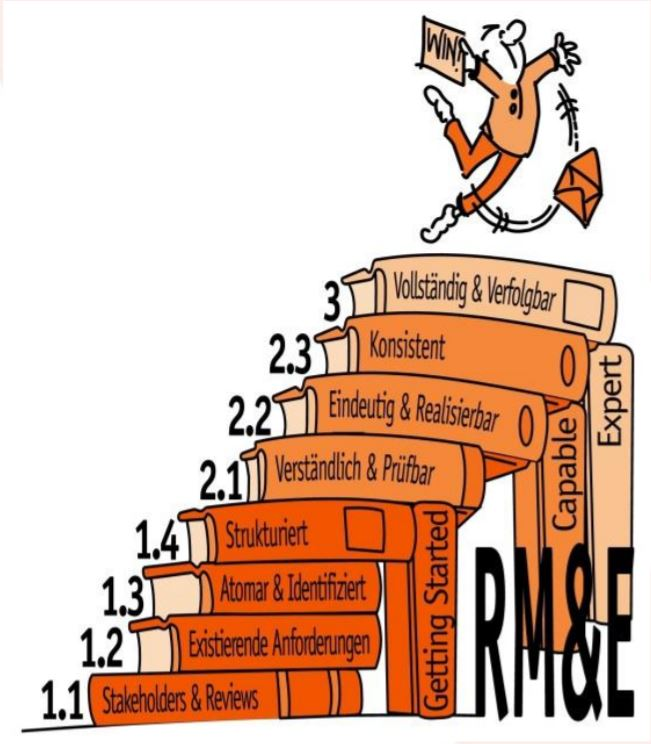
\includegraphics[scale=0.5]{Bilder/HOOD-RE.jpg}
\caption{Überblick der 3 Qualitätsstufen von Anforderungen im \textit{Requirements-Management \& Engineering} (RM \& E) gemäß \cite{hp12}}
\end{center}
\end{figure}

Dabei unterscheidet das Modell zwischen 3 verschiedenen Qualitätsstufen von Anforderungen. Diese werden jeweils durch verschiedene Kriterien dargestellt. Das Ziel der Arbeit der Abteilung bei HELLA stellt demnach das Herstellen einer möglicht hohen Qualitätsstufe der Pflichtenhefte dar. Im besten Fall erreichen die Experten dort die Stufe \textit{Expert} und machen die Anforderungen somit \textit{vollständig \& verfolgbar}.

\subsection{Umgang mit natürlicher Sprache in Lastenheften}
Unvollständige Anforderungen lassen sich meist auf falsche Annahmen der Stakeholder beim OEM zurückführen, die implizite Annahmen bei der Formulierung von Anforderungen treffen und diese Annahmen nicht expliziz erneut aufführen. Ergänzenden Informationen zu Anforderungen können jedoch, wie zuvor gezeigt, durchaus andersartig kategorisiert im Pflichtenheft vermerkt sein. 

Dies resultiert laut \cite{pr15} daher, dass die verschiedenen Autoren des Pflichtenheftes beim OEM als selbstverständlich erachten und diese nicht nochmal für externe Leser hinzufügen. Es stellt sich jedoch die Frage, ob unterschiedliche Menschen jemals ein verlässlich gleiches Verständnis der gleichen Sache haben. 

Colin Hood formuliert Anforderungen grundsätzlich als \glqq individuelle Bedürfnisse\grqq{}, die immer abhängig von dem Autoren sind.\footnote{Im Rahmen unserer Arbeit konnten wir mehrmals Interviews zur Ausrichtung bzw. dem Ansatz unserer Prototypen führen.} In wird die Verwendung von Sprachschablonen für Projektlastenhefte im Vergleich zu natürlicher Sprache evaluiert. Die grundsätzliche Eignung natürlicher Sprache für die Formulierung von Anforderungen wird dort bezweifelt. 

Hood stellte die Eingrenzung der Sprache, die für Projektlastenhefte genutzt werden darf, als eine vielversprechende Möglichkeit vor, sprachliche Eigenheiten der Autoren aus verschiedenen Bereichen effektiv zu vermeiden. Diese Transformation natürlichsprachlicher Anforderungen in formale Sprache als Schablonen stellt auch das Ziel unserer Arbeit dar.

\section{Anwendungsfall bei HELLA} 

Der Anwendungsfall für die zu entwickelnden Werkzeuge ist ähnlich zu dem oben beschriebenen. Es wird davon ausgegangen, dass die HELLA einen Auftrag für ein Produkt von einem OEM erhält. Es ist jedoch bekannt, dass ein ähnliches Produkt, etwa eine frühere Version, bereits von HELLA entwickelt wurde.

Somit liegt ein Pflichtenheft eines OEM in natürlicher Sprache vor. Außerdem existiert zu dem alten Produkt der HELLA bereits in Lastenheft in formalisierter Form.

Ziel ist es die beiden Anforderungsdokumente zu vergleichen um alle Unterschiede der beiden Produkte zu ermitteln. Diese könnten dann etwa genutzt werden um eine sehr frühe und recht präzise Kostenabschätzung der neuen Produktentwicklung an den OEM senden zu können. 

Hierzu muss jedoch zunächst das Pflichtenheft des OEM in eine vergleichbare formalisierte Form gebracht werden. Erst sobald sich also beide Anforderungsdokumente in einer gleichartigen Form befinden kann ein direkter Vergleich der von den Dokumenten beschriebenen Produkte stattfinden. 

Diese Heterogenität von Anforderungsdokumenten ist in der Automobilindustrie vor allem bei der Beziehung zwischen OEM und Zulieferer ein bekanntes und wiederkehrendes Problem.

Daher wird zunächst ein Werkzeug benötigt, welches mit kleinstmöglichem Nutzeraufwand und größtmöglicher Sicherheit ein natürlichsprachliches Anforderungsdokument formalisieren kann. 

Verarbeitet man mit diesem Werkzeug das Pflichtenheft das OEM, so erhält man zwei homogene Dokumente. Hierzu soll außerdem ein Werkzeug entwickelt werden, welches in der Lage ist zwei solcher Dokument zu vergleichen und Unterschiede darzustellen.
\\ 
\newline
HIER USE-CASE ABBILDUNG VON FIRMEN POWERPOINT 
\\
\newline

Die Ansätze und Konzepte solcher Werkzeuge sind in dem folgenden Abschnitt genau beschrieben.

\section[Ansatz und Konzept]{Ansatz und Konzept der Werkzeuge}
Wie bereits unter beschrieben, existiert eine Vielzahl an Arbeiten, die sich mit der verlässlichen Überführung der Anforderungen in natürlicher Sprache in Sprachschablonen beschäftigen. Dazu werden Methoden aus dem NLP und Ontologien genutzt, um den Text der Anforderungen zunächst genau zu annotieren. Dieser Ansatz stellt die Basis für die Vorstellung unseres Werkzeugs in diesem Kapitel dar.

In \cite{zh17} wurde das Potential einer Verbesserung von RE-Prozessen in Firmen durch Werkzeuge aufgezeigt. Die in den vorigen Kapiteln aufgezeigten Anforderungen an das Requirements-Management schaffen somit die Basis für den konkreten Entwurf von Werkzeugen, die entsprechende Funktionalitäten bereitstellen.

\subsection{Anforderungen an die Entwicklung}
Für den Entwurf unserer Prototypen stellt sich einerseits die Frage, an welcher Stelle im abstrakten Modell ein Potential für Werkzeugunterstützung entsteht, auf der anderen Seite aber auch die Definition einer konkreten Zielgruppe bzw. Stakeholdern im tatsächlichen Betrieb bei HELLA, die nachher mit der Software interagieren und diese täglich nutzen.
Für die Entwicklung unseres Werkzeugs haben wir in Zusammenarbeit mit RE-Experten einige Ziele identifiziert, die eine Unterstützung für die Arbeit ausmachen würden:
\begin{enumerate}
\item Zeitersparnis bei Arbeit mit dem Werkzeug, da der Aufwand einer manuellen Prüfung reduziert wird
\item Hoher Automatisierungsgrad bei der Verarbeitung, um Konflikte in den Anforderungen im Voraus aufzulösen
\item Hoher Abdeckungsgrad verschiedener Problemfälle, da eine einfache Wiederverwendbarkeit den Aufwand zur Anpassung an andere Domänen reduziert
\item Mehrwert für den Nutzer, da effektiv Arbeitszeit gespart und Aufwand an das Werkzeug abgegeben werden kann
\item Anforderungen an NLP-Werkzeuge umsetzen, da eine präzise sprachliche Analyse eine wesentliche Grundlage für die Verlässlichkeit der Verarbeitung darstellt.
\end{enumerate}
\subsection{Zuordnung einzelner Werkzeuge}
Verschiedene Verfahren, bereits bei der Spezifikation von Anforderungen im Zusammenhang eines Pflichtengeftes durch Werkzeuge zu unterstützen, sind unter VERWANDTE AREITEN beschrieben. Es existieren jedoch durch die Besonderheiten im geteilten Entwicklungsprozess zwischen OEM und Zulieferer besondere Herausforderungen für das RE, welche Potential für eine Werkzeugunterstützung bieten. 

Wie bereits in Kap. X.X beschrieben, resultieren die Probleme auf Seiten des Zulieferers beim Verständnis der Anforderungen aus dem Umstand, dass dort ein Pflichtenheft in natürlicher Sprache vorliegt. Dieses verursacht einerseits einen Arbeitsaufwand durch die Probleme beim Umgang mit natürlicher Sprache wie z.B. sprachlichen Mehrdeutigkeiten (Kap. X.X). Andererseits können enthaltenen Anforderungen teilweise nicht korrekt bzw. von niedriger Qualität sein, was zu inhaltlichen Probleme für die Produktentwicklung führt. 

Auch kann es mehrere Versionen der Spezifikation eines Produktes im Laufe der Zeit geben, deren Unterschiede erkannt werden müssen. Auswirkungen der Überarbeitung des Produktes auf Basis einer neuen Verison des Pflichtenheftes müssen unter verschiedenen Kriterien gewichtet werden. 

Es gilt also, Werkzeuge zu entwerfen, die insbesondere bei der Lösung von sprachlichen Problemen und bei der Identifikation von Konflikten zwischen Anforderungen in Pflichtenheften unterstützen. 

Daher werden im folgenden die Ansätze aus \cite{zh17} beschrieben, die eine Transformation von bereits spezifizierten Anforderungen in bestehenden Pflichtenheften in eine besser verständliche und eindeutige formale Sprache vorschlagen. Dieser Schritt soll für jedes neu eintreffende Pflichtenheft durchgeführt werden, damit dieses dann standardisiert vorliegt. Die zweite Software-Komponente dient zum automatisierten Vergleich mehrerer verschiedener Pflichtenhefte unter der Verwendung von Ontologien. 

Diese Ansätze haben zur konkreten Entwicklung von zwei Werkzeugen geführt, dem \textit{Requirements-To-Boilerplate-Converter} (R2BC) und dem \textit{Delta-Analyser} (DA). Diese identifizierten Software-Artefakte werden für die Verwendung in einer prototypischen Werkzeugkette hintereinander angeordnet. Somit erfolgt auf Basis der Konvertierung in Schritt 1 die Delta-Analyse in Schritt 2.

\subsubsection{R2BC}
Zu Beginn des Verarbeitungsprozesses liegen die Pflichtenhefte in natürlicher Sprache vor, die der Zulieferer vom Kunden erhalten hat. Im ersten Schritt werden diese natürlichsprachlich formulierten Anforderungen durch den R2BC in Sprachschablonen überführt. 

Nach der Verarbeitung liegt das Pflichtenheft des OEM somit in formaler Sprache vor. Diese Version des Pflichtenheftes kann dann für den Entwicklungsprozess genutzt werden. Das Ziel des R2BC ist es also, die Lesbarkeit bzw. die Eindeutigkeit der Anfordeungen durch Formalisierung zu verbessern. Auf dieser Basis kann dann der Inhalt des Pflichtenheftes eindeutig durch die Entwickler beim Zulieferer verstanden werden. Der Prozess ist in Abb. 3.2 dargestellt.
\begin{figure}[h!]
\begin{center}
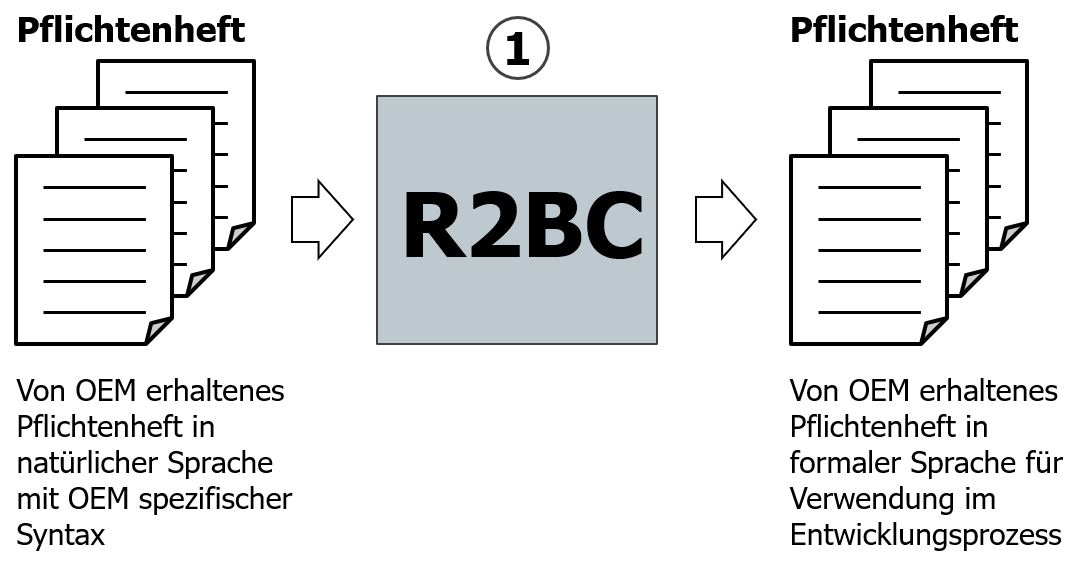
\includegraphics[scale=0.5]{Bilder/Prozess-R2BC.jpg}
\caption{Szenario für Unterstützung durch R2BC-Komponente [eigene Darstellung]}
\end{center}
\end{figure}

\subsubsection{DA}
Diese logisch eindeutige Form der Anforderungen ermöglicht auch einen Vergleich mehrerer Pflichtenhefte anhand der Struktur der einzelnen Anforderungen in einer Ontologie. Diese Unterschiede können durch den DA identifiziert und in Form eines Deta-Reports ausgegeben werden. Unterschiede können anschließend etwa für einen RE-Experten auf dem Bildschirm bzw. in eine Datei ausgegeben werden. Der Ablauf ist in Abb. 3.3 dargestellt.
\begin{figure}[h!]
\begin{center}
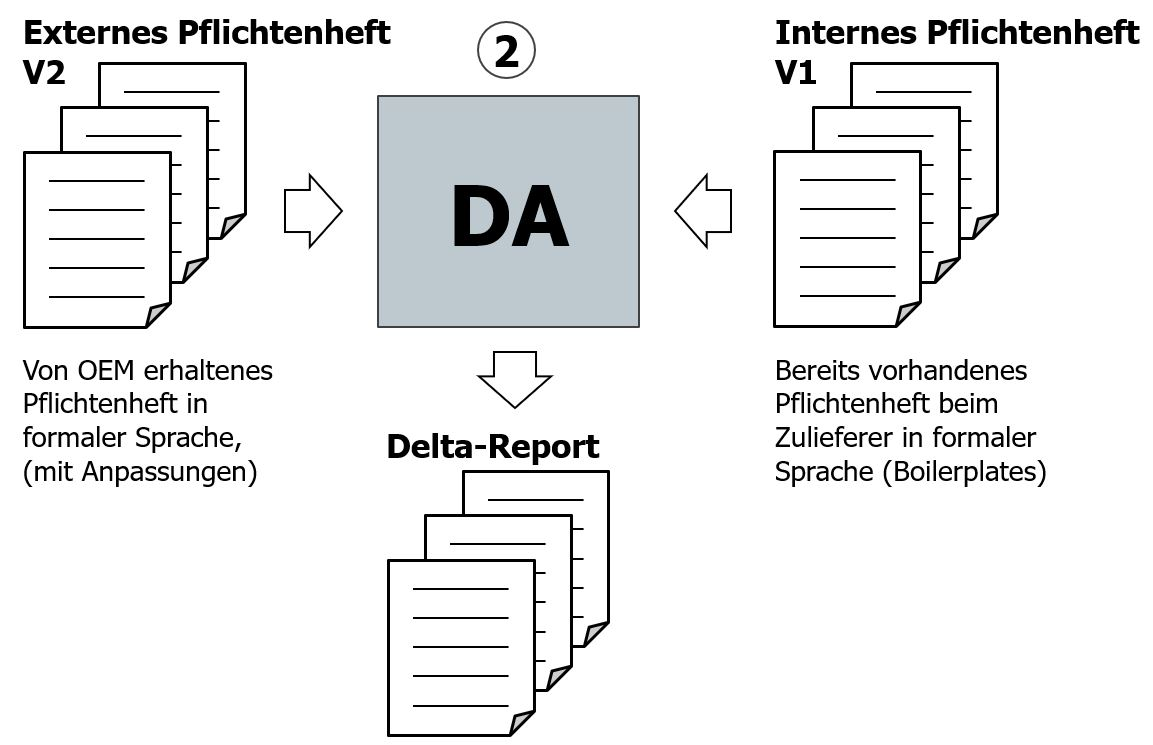
\includegraphics[scale=0.5]{Bilder/Prozess-DA.jpg}
\caption{Szenario für Unterstützung durch DA-Komponente [eigene Darstellung]}
\end{center}
\end{figure}

Alternativ können Änderungen auch automatisiert durch eine Integration der Anpassungen in das interne Pflichtenheft übernommen werden. Dazu müssen im Programm Verfahren zur Gewichtung der Deltas bzw. Metriken zur Entscheidung zwischen Anforderungen hinterlegt sein.

Angesichts der Aufgaben für die Werkzeuge stellt sich die Frage nach dem erreichbaren Grad der Automatisierung bei hoher Verlässlichkeit im Gegensatz zu möglichen erforderlichen Interaktionspunkten mit dem Nutzer. 

Der prinzipielle Aufbau beider Werkzeuge wird in den folgenden Abschnitten beschrieben.

\subsection{R2BC-Funktionalität}
Wie bereits zuvor beschrieben wurde, stellt der \textit{Requirements-To-Boilerplate-Converter} die erste wesentliche Stufe bei der automatisierten Verarbeitung von Pflichtenheften dar. Die Textverarbeitung erfolgt dabei sukzessive bzw. satzweise aus dem Quelldokument in ein Zieldokument, dass am Ende alle Anforderungen in angepasster Form enthält. 

Dabei greift er auf eine formale Sprache zurück, die in verschiedenen Schablonen repräsentiert und im Programm gespeichert ist. Diese eingeschränkte Sprache ist Zulieferer-intern fest dokumentiert und wurde zuvor durch RE-Experten eindeutig definiert, was zu einer verbesserten Verständlichkeit führt. Sprachschablonen stellen demnach, im Kontrast zu natürlicher Sprache, eine eindeutige Deutung der Anforderungen sicher. Im besten Fall wurden somit insbesondere sprachliche Mehrdeutigkeiten im Sinne der Atomarität von Anforderungen eliminiert bzw. aufgeschlüsselt.

Der R2BC verarbeitet die Pflichtenhefte unter Zugriff auf diese formalen Sprachschablonen (\textit{Boilerplates}) automatisiert und ein Eingreifen des Nutzers ist nur im Ausnahmefall erforderlich. 

\subsubsection{Programmablauf und Artefakte}
Auf Basis dieses Ansatzes wurde ein Algorithmus zur satzweisen Verarbeitung der Sätze unter Verwendung des NLP-Werkzeugs GATE entwickelt, der aus natürlichsprachlichen Eingaben (Input) eine Ausgabe (Output) in formaler Sprache erzeugt. Dabei werden auch Metainformationen über den Text generiert und zur weiteren Verarbeitung ausgegeben.

Der prinzipielle Programmablauf gliedert sich wie folgt:
\begin{enumerate}
\item Zunächst werden die Sätze für eine sukzessive Verarbeitung getrennt. Dies erfolgt mithilfe des NLP-Werkzeugs GATE.
\item Für jeden Satz wird geprüft, ob und in welchem Maße Anpassungen an die formale Sprache der Boilerplates erforderlich sind. Dazu werden Syntax bzw. Satzbestandteile analysiert.
\item Passende Boilerplate-Typen für die Anforderung wird identifiziert. Dieser leitet sich aus den unter 2. gefundenen Merkmalen ab. Es können etwa funktionale von nicht-funktionalen unterschieden sowie Bedingungen für die Anforderung modelliert werden.
\item Sind Anpassungen erforderlich, so wird eine Konvertierung in die jweils passende Boilerplate durchgeführt und diese werden im Programm gesammelt. 
\item Die erzeugte Boilerplate, die am besten zum Inhalt der Anforderung passt, wird identifiziert. Dies kann automatisiert oder unter Einbezug des Nutzers geschehen. Der Nutzer kann dazu beispielsweise aus mehreren Vorschlägen auswählen.
\item Sind alle Anforderungen aus dem Quelldokument verarbeitet, wird auf Basis der erzeugten Anforderungen in Boilerplates ein Zieldokument für die weitere Verwendung erzeugt.
\end{enumerate}

Auf Basis dieses Konzeptes wurde in QUELLE PAPER ein Vorschlag zur Aufteilung der Ressourcen in verschiedene Bereiche gemacht. Dabei gliedern sich die Funktionalitäten in drei Software-Komponenten, die in Abb. 3.4 dargestellt sind.
\begin{figure}[h!]
\begin{center}
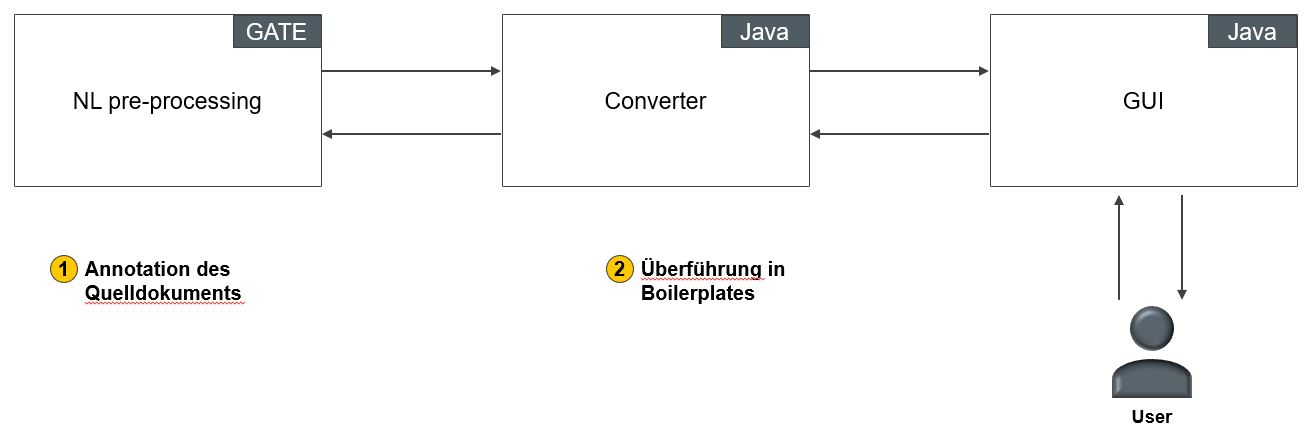
\includegraphics[scale=0.5]{Bilder/Verteilung-R2BC.jpg}
\caption{Verteilung der R2BC-Ressourcen [eigene Darstellung]}
\end{center}
\end{figure}
Der Programmablauf ist durch die Schritte 1 und 2 grob dargestellt und verteilt sich hauptsächlich auf die zwei entsprechenden Artefakte. Die Komponenten lassen sich dabei wie folgt definieren:
\begin{itemize}
\item Die \textit{NL pre-processing} Komponente stellt das backend für die Sprachverarbeitung des Quelldokumentes dar. Dabei werden verschiedene Textbereiche mithilfe des NLP-Werkzeugs GATE annotiert und somit relevante Informationen über den Text generiert. Das Ziel ist es, konkrete Anforderungen im Pflichtenheft eindeutig zu identifizieren. GATE stellt ein in hohem Maße konfigurierbares Werkzeug auf \textit{java}-Basis dar, dass in Kap. 4.1 näher beschrieben wird.
\item Die zweite Komponente beinhaltet die Konvertierung der Sätze aus dem Quelldokument in Sprachscablonen. Der \textit{Converter} nutzt dabei die zuvor erstellten Annotationen, um für jeden Satz im Anforderungsdokument eine oder mehrere passende Sprachschablonen zu finden. Diese Schablonen werden dann durch das Programm generiert bzw. passend \glqq befüllt\grqq{}. Der \textit{Converter} wird ebenfalls mit \textit{java} implementiert.
\item Die Interaktion mit dem Nutzer wird durch ein herkömmliches \textit{GUI} realisiert, dass dem Nutzer die Navigation im Programm ermöglicht. Auch kann dort etwa die Anzeige und Auswahl von einer aus mehreren möglichen Konvertierungen erfolgen.
\end{itemize}

In Kap. 4 erfolgt auf dieser Basis die konkrete Implementierung eines Prototypen für den R2BC.
\subsection{DA-Funktionalität}
Auf Basis des zuvor beschriebenen R2BC stellt der \textit{Delta-Analyser} die Softwarekomponente für einen kriteriengeleiteten Vergleich zweier Anforderungsdokumente dar. Das Ziel ist es, auf Basis der Informationen zu jeweils einem der Lastenhefte den Grad der inhaltlichen Überschneidung zum anderen Lastenheft zu messen. 

Im Kontext des Use-Cases dieser Arbeit geht es dabei insbesondere um den Vergleich von zwei Versionen des gleichen Anforderungsdokumentes, wenn auf Unterschiede in der Überarbeitung geprüft werden soll. Zu Anforderungen aus dem Lastenheft V2 müssen also inhaltlich passende Anforderungen aus Lastenheft V1 gefunden werden, um anschließend Deltas zwischen diesen Anforderungen zu identifizieren bzw. für den Nutzer hervorzuheben. Diese Verarbeitung erfolgt dabei satzweise für das komplette Lastenheft. 

Für ein automatisiertes Finden passender Requirements in unserem Werkzeug müssen daher die Anforderungen in einheitlicher Form dargestellt sein, damit verlässlich nach einzelnen Satz- bzw. Textbestandteilen in den Anforderungen gesucht und verglichen werden kann.
Dabei stellt, wie zuvor beschrieben, die Überführung der Anfordeurngen aus den Dokumenten aus der natürlichen in eine fest definierte, formale Sprache, eine wesentliche Grundlage dar. Der zuvor skizzierte R2BC bietet eben diese Funktionalität.

\subsubsection{Programmablauf und Artefakte}
Die bechriebenen Funktionen ermöglichen den Entwurf eines Verfahrens für einen automatisierten Vergleich von zwei Lastenheften im DA. Dazu wird jede Anforderungen aus dem Lastenheft V2 mit denen aus V1 abgegelichen, um jeweils zueinander passende zu finden.
Folgendes Vorgehen wurde dazu entwickelt:
\begin{enumerate}
\item Die einzelnen Anforderungen in Boilerplates werden für Lastenheft V1 und V2 geladen.
\item Für jede Boilerplate aus Lastenheft V2 wird geprüft, ob es identische, vergleichbare oder keine zuordbaren Anforderungen in Lastenheft V1 gibt. Diese drei Kategorien werden auf Basis der GATE-Annotationen aus dem R2BC identifiziert.
\item Entsprechend des gefundenen Überinstimmungsgrades werden die Deltas zwischen den Anforderungen identifiziert:
\begin{enumerate}
\item \textit{Identische Anforderung}: Es wurde eine identische Anforderung in beiden Lastenheften gefunden. Die Anforderung kann ohne gesonderte Betrachtung übernommen werden.

\item \textit{Verglichbare Anforderung}: Es wurden nur eine teilweise übereinstimmende Anforderung gefunden. Dies ist etwa der Fall, wenn sich Anforderungen geändert haben bzw. überarbeitet wurden. Zwischen diesen Anforderungen existiert also ein Delta, das eine Änderung in den Anforderungen signalisiert und somit den Produktspezifikationen bedeuten würde. 

Eine feingranulare Aufschlüsselung der erwartbaren Deltas findet sich in der Implementierung in Kap. 4.x. Dort werden auch Vorschläge zur Gewichtung verschiedener Deltas im Kontext des RE gemacht.

\item \textit{Keine vergleichbare Anforderung}: Es konnte keine Anforderung aus V1 gefunden werden. In Lastenheft V2 könnten etwa neue Anforderungen enthalten sein, die in V1 noch in keiner Weise spezifiziert wurden. Dies kann etwa Eigenschaften betreffen, die erst später im Entwicklungsprozess definiert wurden oder zu der vorher noch keine Informationen bekannt waren. Im Kontext anderer Anforderungen muss dabei auf Konsistenz geprüft werden.

\end{enumerate} 
\item Falls es noch mehr mindestens vergleichbare Anforderungen in V1 gibt, wird die am besten passende Anforderung gefunden. 
\item Der Delta-Report für den Nutzer wird unter Zugriff auf die Ergebnisse aus 4. erzeugt, wenn V2 vollständig durchlaufen wurde.
\end{enumerate}
Insofern Deltas gefunden wurden, muss immer auch die Umsetzbarkeit dieser neuen Anforderungen gesondert geprüft werden. Die weitere Korrektheit des Lastenheftes V2 zu V1 kann bei vielen Deltas nicht gewährleistet werden, was eine Umsetzung der Anforderungen erschwert. Es können massive Unterschiede in den Spezifikationen auftreten, was zu einer teilweisen oder kompletten Neuentwicklung des Produktes führen kann.

Die beschriebene Funktionalität hat in der Entwicklung unseres Werkzeugs zur konkreten Herausbildung von drei Kernbestandtreilen geführt. Unser Werkzeug beinhaltet dabei Komponenten zur Abbildung von Fachlogik und GUI. Die Verteilung der Ressourcen ist in Abb. 3.4 dargestellt. 
\begin{figure}[h!]
\begin{center}
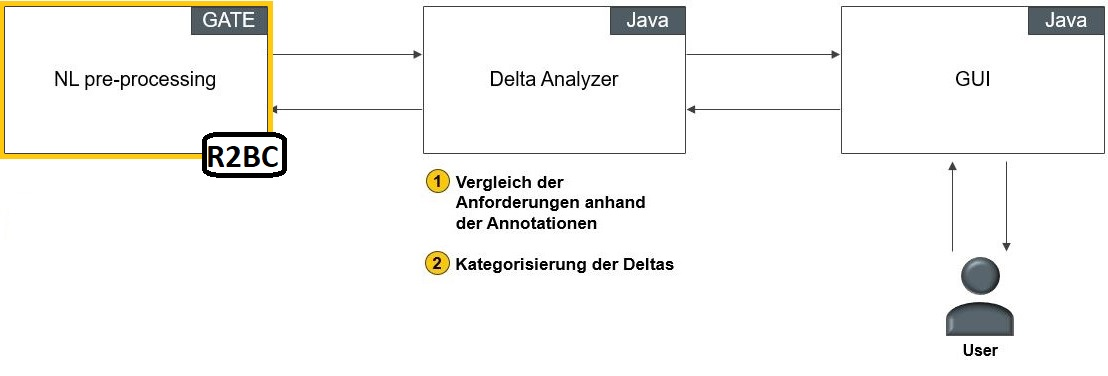
\includegraphics[scale=0.6]{Bilder/Verteilung-DA.jpg}
\caption{Verteilung der DA-Ressourcen [eigene Darstellung]}
\end{center}
\end{figure}
Die Komponenten realisieren dabei die zwei Hauptfunktionalitäten 1 und 2 in Form von GATE und java-Ressourcen. Auf dieser Basis können den einzelnen Komponenten Funktionalitäten wie folgt zugeordnet werden:
\begin{itemize}
\item \textit{NL-pre-processing} Wie schon beim R2BC dient diese Komponente zur Generierung von Informationen über den annotierten Text. Da der DA die zweite Stufe der Verarbeitung darstellt, nutzen wir hierzu die Ergebnisse aus dem R2BC, d.h. die dort generierten Annotationen, die wir in den DA einlesen. Somit können die Anforderungen, die nach dem R2BC in Boilerpaltes vorliegen, anhand ihrer Annotaionen verglichen werden.
\item Der \textit{Delta-Analyser} prüft die verschiedenen Anforderungen aus Pflichtenheft V2 auf ihren Übereinstimmungsgrad mit den Anforderungen aus V1. Dabei greft er auf die geladenen Annotationen beider Pflichtenhefte zu und vergleicht daran verschiedene Anforderungen. Schlussendlich wird ein Delta-Report erstellt, der alle Deltas zwischen den Anforderungen enthält.
\item Die \textit{GUI} ermöglicht dem Nutzer die Eingabe der zwei zu vergleichenden Pflichtenhefte. Nach der Verarbeitung erhält der Nutzer dort eine Übersicht der Unterschiede der beiden Pflichtenhefte, indem die jeweils verglichenen Anforderungen dort angezeigt werden.
\end{itemize}
Die Implementierung des DA auf Basis des zuvor implementierten R2BC ist in Kap. 5 beschrieben. Dort werden auch konkrete Erweiterungen und Verbesserungspotentiale des Programms beschrieben, die nach der Entwicklung identifiziert wurden.


\chapter{Requirements-To-Boilerplate-Converter (R2BC)}
Dieses Kapitel behandelt den \textit{Requirements-to-Boilerplate-Converter} (\textit{R2BC}) ausführlich. Hierzu wird zunächst der Aufbau des Tools aus den verschiedenen Klassen und der verwendeten Software beschrieben. Daraufhin wird die Implementierung wichtiger Funktionalitäten und Datenstrukturen mit Auszügen des Quellcodes gezeigt und erläutert. Anschließend wird das Testverfahren für das Werkzeug beschrieben und die dadurch erzielten Ergebnisse aufgeführt. Die Evaluation der Ergebnisse findet in einem späteren Kapitel statt. Abschließend wird ein Katalog mit möglichen Erweiterung und Verbesserungen für das Werkzeug geliefert, welche auf Grund mangelnder Zeit und Ressourcen von uns nicht mehr umgesetzt werden konnten. 

\section{Architektur, Klassen und Verteilung der Ressourcen}
In diesem Abschnitt soll die Architektur des R2BC vorgestellt und erläutert werden. Dazu gehört die zur Entwicklung verwendete Software, sowie ein Überblick über die Klassenstruktur des Werkzeugs. 

\subsection{Verwendete Software}
Als verwendete Software werden sämtliche Programme aufgeführt, welche eine Hilfe bei der Implementierung oder Teile der Funktionalität des Programmes darstellen. 

\subsubsection{Implementierungsunterstützung}
Das Werkzeug wurde auf Basis der Programmiersprache JAVA geschrieben. Hierzu wurde das JDK (\textit{JAVA development kit}) 8.1 verwendet. 

Die Wahl der Programmiersprache fiel aufgrund von zwei Hauptfaktoren auf JAVA: 
\begin{enumerate}
\item JAVA ist eine weit verbreitete und entwicklerfreundliche Programmiersprache. Vorteile der Sicherheit von JAVA werden außerdem in \cite{rs18} aufgeführt.
\item Das Programm, welches für das NLP-Preprocessing verwendet wird ist JAVA-basiert. Somit fällt die Integration des Programms in unser Werkzeug einfacher. Dies wird jedoch noch genauer in einem späteren Abschnitt behandelt.
\end{enumerate}

Als Programmierumgebung\footnote{oft als IDE, also \textit{integrated development enviroment} bezeichnet} wurde die Netbeans 8.2 IDE verwendet. Diese mit mit \textit{Eclipse} eine der am weitesten verbreitete Programmierumgebung für JAVA-Programme. 

Außerdem wurde die Software \textit{Apache Maven} als Build-Management-Tool (\textit{BMT}) verwendet. Dieses wird vor allem für JAVA-Programme verwendet und war daher sehr geeignet für die Verwendung in unserem Werkzeug. Außerdem wurde das selbe BMT auch in dem später beschriebene Tool zur Bereitstellung bestimmter Funktionalitäten verwendet. 
Build-Management-Tools helfen grundsätzlich dabei bestimmte, zuvor nicht vorhandene Bibliotheken und deren Funktionalitäten nachzuladen und in ein Programm zu integrieren. Außerdem helfen sie bei dem späteren Ausliefern des Programms, also der Erstellung eines unabhängig ausführbaren Programms außerhalb der Programmierumgebung.
In unserem Fall wurde also eine \textit{Executable JAR} (ausführbares JAVA-Archiv) erstellt. 

\subsubsection{Funktionalitätsunterstützung}

Das zuvor bereits erwähnte Programm zur Bereitstellung von Funktionen ist bekannt unter dem Namen GATE (\textit{General Architecture for Text Engineering}). Dies ist ein Werkzeug zur Erstellung von NLP-Programmen und wird ausführlich in \cite{rs18} behandelt. 

In unserem Programm wird \textit{GATE Embedded} verwendet. Dies ist eine Ansammlung von JAVA-Bibliotheken, welche alle Funktionen von GATE bieten. Man erhält also das gesamte Programm, nur ohne Benutzeroberfläche. Im folgenden wird daher im Zusammenhang auf die entwickelten Werkzeug nicht zwischen GATE und GATE Embedded unterschieden. 

GATE ist, wie in Abbildung X.X (Konzept) zu sehen ist, für das NLP, also die Sprachverarbeitung in unserem Werkzeug zuständig und bildet somit das \textit{Backend} des Programms.

Die genaue Umsetzung vom NLP in unserem Programm und der damit verbundene Einsatz von GATE sind jedoch Teil der Implementierung und werden somit in Abschnitt X.X behandelt.

\section{Klassenstruktur}
Im Rahmen der Entwicklung unseres Proof-of-concepts wurde die Funktionalität aus Kap. 3.x auf verschiedene Komponenten aufgeteilt. Hier soll lediglich ein grober Überblick der Ressourcenverteilung im Programm gegeben werden, der Programmablauf findet sich in Kap. 4.x.

Verschiedene Programmbausteine sind dabei modular aufgebaut und verteilen sich auf die Pakete \textit{R2BC}, der die Fachlogik enthält, \textit{R2BCGUI}, das eine simple GUI-Klasse enthält, und \textit{Boilerplates}, das die Objekte zur Erzeugung von Sprachschablonen enthält (siehe Abb. 4.x).

\begin{figure}[h!]
\begin{center}
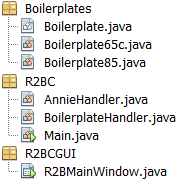
\includegraphics[scale=1.0]{Bilder/R2BC-Pakete.png}
\caption{Zuordnung der R2BC-Klassen zu Paketen nach Abb.3.x [eigene Darstellung]}
\end{center}
\end{figure}

Die Funktionalität wurde dabei hauptsächlich mit verschiedenen java-Klassen umgesetzt, die die Umsetzung der Fachlogik darstellen. Die Anbindung an das NLP-Werkzeug GATE-Embedded erfolgte dabei unter Verwendung verschiedener java-Bibliotheken, die extern im Programmordner gespeichert sind. Die GATE-Ressourcen wurden dabei zur Annotation von Text genutzt, die selbst entwickelten java-Klassen einerseits für die GATE-Konfiguration, andererseits für die Auswertung der dort erstellten Annotationen. 

\begin{figure}[H]
\begin{center}
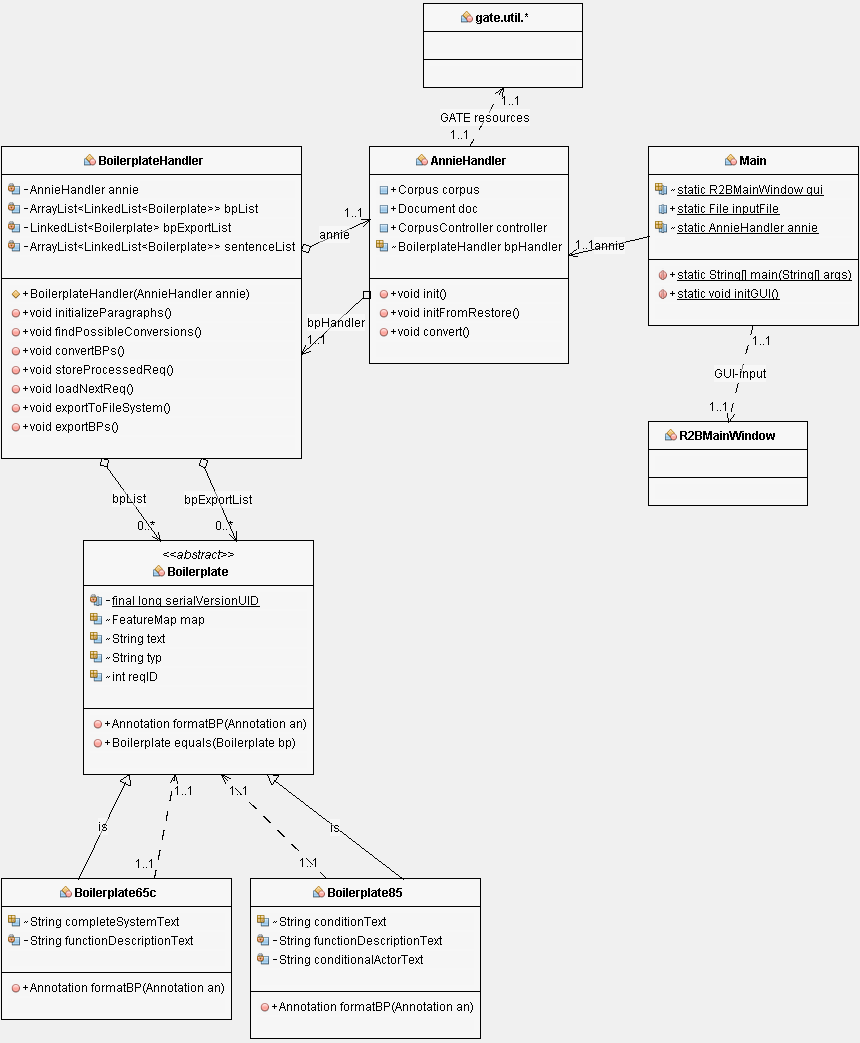
\includegraphics[scale=0.57]{Bilder/r2bc-klassen.png}
\caption{Klassendiagramm R2BC [eigene Darstellung]}
\end{center}
\end{figure}

Auf Basis des in Kap. 3.x beschriebenen Algorithmus können die Aufgaben der verschiedenen Klassen in Abb. 4.x wie folgt erläutert werden:\footnote{Die Darstellung der GUI-Klasse in Abb. 4.x ist für eine bessere Übersichtlichkeit vereinfacht worden. Enthaltene Objekte und Funktionalitäten beziehen sich dabei jedoch nur auf die GUI-Elemente.}

\begin{itemize}
\item \textit{Main -} Die Hauptklasse ermöglicht den Zugriff auf alle Funktionen des Programms. Es erfolgt die Initialisierung aller Programmkomponenten. Es werden dazu verschiedene Objekte für die Textverarbeitung (\textit{AnnieHandler}, \textit{BoilerplateHandler}) sowie für die GUI (\textit{R2BMainWindow}) erzeugt. Hauptsächlich dient die Hauptklasse auch der Initialisierung der GUI, um die dortigen Schaltflächen mit Funktionen zu belegen. In der GUI ist beispielsweise ein Button zum Starten der Konvertierung enthalten, der eine Funktion des BoilerplateHandler aufruft. 
\item \textit{AnnieHandler -} Der Annie-Handler realisiert den Zugriff auf die Bestandteile der Sprachverarbeitung aus dem Werkzeug GATE. Hauptsächlich betrifft dies die Verarbeitungslogik ANNIE, die konkrete Komponenten zur Textverarbeitung enthält (siehe Abschnitt 4.x). Im AnnieHandler werden dazu neben den Verarbeitungswerkzeugen auch die Textressourcen, die im Programm verarbeitet werden sollen, initialisiert. Diese \textit{Language-Ressourcen} aus GATE beinhalten neben dem Text auch alle generierten Annotationen. Der AnnieHandler beinhaltet nach der Verarbeitung somit alle Informationen zu den Anforderungen in einer Liste. Auf Basis dieser Informationen kann dann die Transformation von Anforderungen in Boilerplates im \textit{BoilerplateHandler} erfolgen.
\item \textit{BoilerplateHandler -} Die Klasse dient der Erzeugung von jeweils passenden Boilerplates zu einer Anforderung, indem aus dem Text alle relevanten Informationen zur Erzeugung passender Boilerplates extrahiert werden. Der BoilerplateHandler beinhaltet dazu sowohl Funktionen zur Identifikation passender Boilerplates auf Basis der Annotationen aus der GATE-Verarbeitung, als auch die Erzeugung von konkreten Boilerplate-Objekten aus der abstrakten Klasse Boilerplate, wenn die passenden Annotationen dazu gefunden wurden.
\item \textit{Boilerplate -} Die Klasse bündelt alle Kernmerkmale der Boilerplates, die durch das Programm erzeugt wurden. Dies betrifft in erster Linie den Gesamttext, die einzelnen Satzbestandteile und Metainformationen über die Anforderung, wie etwa eine ID.
\item \textit{Boilerplate65c} und \textit{Boilerplate85 -} Wie bereits unter 3.x beschrieben, wurden im Zuge der Entwicklung dieses Werkzeugs zwei prototypische Boilerplates implementiert. Diese konkreten Boilerpalte-Objekte beinhalten eine Repräsentation der GATE-Annotation einzelner Satzbestandteile als Zeichenketten, um daraus ganze Sätze zu erzeugen. Der Boilerplate-Handler "befüllt" somit konkrete Boilerplates mit allen erforderlichen Begriffen anhand der dort definierten Bestandteile.
\begin{itemize}
\item Die Klasse \textit{Boilerplate65c} stellt eine Schablone für Systemfunktionen dar und enthält demnach Platzhalter für ein System und eine Funktion dieses Systems, die dann bei der Erzeugung konkreter Boilerplate-Objekte in das Grundgerüst des Satzes eingefügt werden. Typ 65c Boilerplates sehen demnach etwa so aus: 

\tt
The complete system <<System>> shall perform \\
<<FunctionDescription>>.\footnote{<<System>> und <<FunctionDescription>> werden durch die Verarbeitung des Satzes in GATE eindeutig anhand passender Annotationen identifiziert und zugeordnet. Der Rest des Satzes ist fest hinterlegt.}
\rm

\item Die Klasse \textit{Boilerplate85} stellt vereinfacht eine Erweiterung der Boilerplate65c um eine Bedingung dar. Dementsprechend existiert auch hier ein System und eine Funktion, aber auch eine Bedingung, unter der die Funktion ausgeführt wird. Diese drei Bestandteile werden für die Erzeugung von Typ 85 Boilerplates benötigt. Das Grundgerüst der Sätze mit bedingten Funktionen sieht dabei wie folgt aus:

\tt
Under the condition: <<conditionText>> the actor: \\
<<conditionalActorText>> shall \\
<<functionDescriptionText>>.\footnote{Eine Unterscheidung zu Typ65c scheint zunächst nicht trivial, da conditionText auch einfach leer sein kann und somit Typ 65c fälschlicherweise als Typ 85 erzeugt werden können. Durch die unterschiedliche ANnotation der beiden Typen schon bei der GATE-Verarbeitung kann dennoch eine verlässliche Unterscheidung erfolgen.}
\rm
\end{itemize}

\end{itemize}
Die Funktionalität des Gesamtprogramms, das sich aus dem Zusammenspiel der KOmponenten ergibt, ist in den folgenden Abschnitten dargestellt.


\section{Werkzeug-Implementierung}
In diesem Abschnitt werden wichtige Aspekte der praktischen Umsetzung des Programms genau erläutert. Die bezieht sich sowohl auf präzisere Vertiefung der Konzepte, also auch Quellcode-Beispiele der Implementierung zur Erläuterung des Programmvorgehens und die daraus resultierenden Interaktionsmöglichkeiten der Benutzer.  
\subsection{Sprachverarbeitung mit GATE}
Dieser Abschnitt beschäftigt sich mit der automatischen Sprachverarbeitung der Anforderungsdokumente mit Hilfe des angekündigten NLP-Werkzeugs \textit{GATE}. Dies beinhaltet, das Einlesen der Lastenhefte, die Erstellung einer Verarbeitungslogik, die Erstellung und Auswertung von Verarbeitungsregeln und das Einbinden von GATE in das spätere Programm. Fokus liegt dabei auf der praxisnahen Verwendung in dem Projekt. Ein genereller Überblick und Einordnung des Werkzeugs finden sich in der vorherigen Arbeit \cite{rs18}.

\subsubsection{Einlesen von Lastenheften}
In GATE benötigt man zum einlesen und verwenden von Dokumenten zunächst einen \textit{Corpus}, also einen Textkörper. Dieser kann später mehrere Dokumente enthalten und diese verwalten. Außerdem wird eine Verarbeitungslogik immer auf einem Korpus (nicht auf einem Dokument) ausgeführt. Im Zusammenhang dieser Arbeit war es nicht nötig einen Corpus mit verschiedenen Dokumenten zu befüllen, daher ist zukünftig die Verarbeitung eines Corpus gleichbedeutend mit der Verarbeitung eines Dokuments. 

Ein Corpus kann in der Benutzeroberfläche von GATE schnell als neue \textit{language resource} (Sprachliche Ressource) erzeugt werden. In GATE Embedded ist dies ohne Benutzeroberfläche natürlich nicht möglich, lässt sich jedoch ähnlich einfach durch den Aufruf von \textit{new Corpus} durchführen. 

Sobald der Corpus erstellt ist, lassen sich dort Dokumente einfügen. \footnote{Alternativ kann auch erst ein Dokument eingelesen und anschließend ein Corpus um dieses angelegt werden.} Auch dies geschieht in GATE direkt über die Benutzeroberfläche. In GATE Embedded verwendet man hierzu den \textit{add}-Aufruf eines Corpus-Objekts mit einem übergebenen Dokument. 

Sobald man einen Corpus mit mindestens einem Dokument hat, kann man auf diesem Corpus eine Verarbeitungslogik aufrufen (oft auch Verarbeitungs-Pipeline genannt, wegen der Aneinanderreihung mehrerer Verarbeitungskomponenten). Diese werden im folgenden Abschnitt genauer beschrieben.

\subsubsection{GATE-Verarbeitungslogik}
In GATE wird die sprachliche Analyse durch eine Verarbeitungslogik durchgeführt, welche aus verschiedene Verarbeitungsressourcen (\textit{processing resource}) aufgebaut ist. Eine Standard-Verarbeitungslogik wird durch das GATE-Plugin \textit{ANNIE} zur Verfügung gestellt. Die einzelnen ANNIE-Verarbeitungsressourcen sind in \cite{rs18} beschrieben. 

Führt man eine Verarbeitungslogik auf einem Corpus bzw. auf dessen Dokumenten aus, so werden durch die verschiedenen Verarbeitungsressourcen an bestimmten Stellen im Text bestimmte Informationen hinzugefügt. Dies bezeichnet man als \textit{annotieren}. Dabei wird der Text an sich nicht geändert, die Annotationen können jedoch etwa durch farbige Unterlegung des betroffenen Texts in der GATE-Benutzeroberfläche gezeigt und als XML-Datei exportiert werden. 

\begin{figure}[H]
\begin{center}
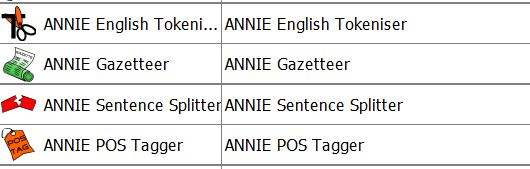
\includegraphics[scale=0.9]{Bilder/ANNIEinGATE.jpg}
\caption{Anforderung mit farbig markierten Token-Annotationen in GATE}
\end{center}
\end{figure}   

Einer Annotation können sog. \textit{Features} also Eigenschaften zugewiesen werden, welche dann noch weitere Informationen enthalten können, wie z.B. Länge der Annotation und die betroffene Zeichenkette.

\begin{figure}[H]
\begin{center}
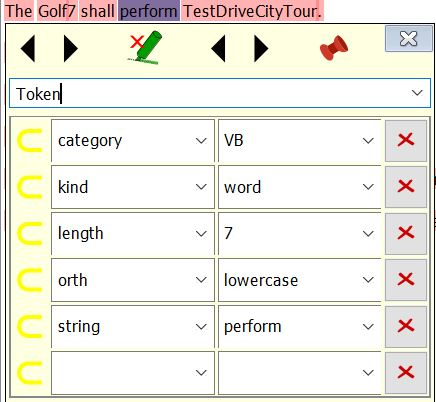
\includegraphics[scale=0.9]{Bilder/FeaturesInGATE.jpg}
\caption{Ausgewählte Token-Annotation und dessen Features in GATE}
\end{center}
\end{figure}  

Die für diese Arbeit verwendeten und besonders relevanten ANNIE- Verarbeitungsressourcen und die dadurch entstehenden Annotationen sind: 


\begin{enumerate}
\item \textit{ANNIE Tokenizer}: Der Tokenizer unterteilt den Text oberflächlich in Zeichen oder Zeichenketten, welche als Zahlen, Wörter (Groß- und Kleinschreibung wird unterschieden) und Interpunktion kategorisiert werden. Dies fügt an den betroffenen Stellen die \textit{Token}-Annotation hinzu, welche jeweils Typ (Zahl, Wort usw.) und Länge in Zeichen . Die Verarbeitung durch den Tokenizer soll so effizient wie möglich sein und nur als Grundlage etwa für spätere Grammatikregeln dienen.

\item \textit{ANNIE Gazetteer}: Ein Gazetteer beinhaltet relevante Eigennamen aus bestimmten Bereichen. Es handelt sich dabei um eine geschachtelte Liste, welche für jeden Bereich (beispielsweise Städte, Flughäfen, Fußball Clubs) über eine Liste der jeweils bekannten Eigennamen verfügt. Gazetteers werden verwendet, um domänenspezifisch Entitäten zu erkennen, da diese in einem normalen Wörterbuch nicht zu finden sind. Die vorgefertigten Listen sind also je nach Dokument individuell zu erweitern bzw. zu erstellen. Wird ein Listenelement im Text wiedererkannt, so erhält es Standardmäßig die \textit{Lookup}-Annotation. Das lässt sich jedoch auch schon im Gazetteer ändern und jeweils Listen-abhängig bestimmen. 

\item \textit{ANNIE Sentence Splitter}: Der Sentence-Splitter unterteilt den gesamten Text in einzelne Sätze. Dadurch wird jeder komplette Satz von einer \textit{Sentence}-Annotation umschlossen. Dies wird später für den Part-of-Speech Tagger benötigt. Der Splitter verwendet dazu einen Gazetteer mit Abkürzungen, um Interpunktion wie etwa Fragezeichen, Ausrufezeichen und Punkte von anderen Sonderzeichen wie Semikola und Doppelpunkten zu unterscheiden. 

\item \textit{ANNIE POS Tagger}: Der Part-of-Speech Tagger annotiert alle Wörter und Symbole gemäß ihrer grammatikalischen Funktion. Hierfür wird keine neue Annotation angelegt, es werden jedoch das wichtige \textit{category}-Feature an die Token-Annotationen angefügt. Dies ist wichtige Grundlage für grammatikalische Analyse von Sätzen. Dazu gehören Dafür nutzt dieser Standard-Lexika und Regelwerke, welche auf dem Corpus-Training des Wall Street Journal beruhen.
\end{enumerate}

\begin{figure}[H]
\begin{center}
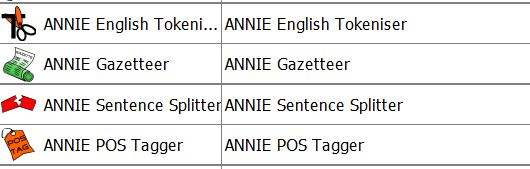
\includegraphics[scale=0.9]{Bilder/ANNIEinGATE.jpg}
\caption{Verwendete ANNIE-Verarbeitungsressourcen in GATE [eigene Darstellung]}
\end{center}
\end{figure}   

\subsubsection{JAPE Transducer}

Die für die Verarbeitung wichtigsten Komponenten sind in der normalen ANNIE-Verarbeitungslogik jedoch noch nicht vorhanden. Die sogenannten \textit{JAPE Transducer} werden individuell angelegt und verwenden die Annotationen der vorherigen Verarbeitungsressourcen, um dem Text wichtige Informationen hinzuzufügen. Diese können im Gegensatz zu den vorherigen jedoch auch von großer inhaltlicher bzw. semantischer Relevanz sein. Jape Transducer lassen sich wie die anderen Verarbeitungsressourcen hintereinander reihen und somit in eine Verarbeitungslogik einfügen.

\begin{figure}[H]
\begin{center}
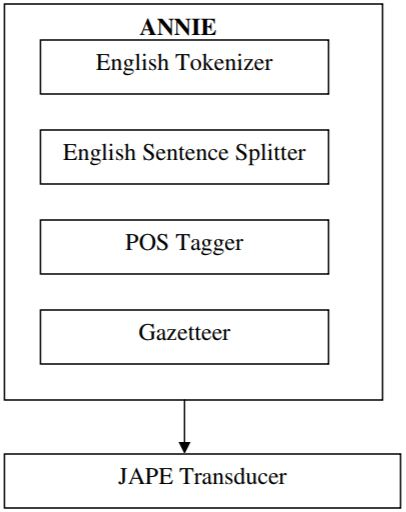
\includegraphics[scale=0.7]{Bilder/ANNIE-Pipeline.jpg}
\caption{Verarbeitungslogik aus ANNIE und JAPE Transducern \cite{tol09}}
\end{center}
\end{figure}   

In JAPE-Transducern\footnote{sowie in einigen der anderen Verarbeitungsressourcen} wird die im Namen vorhandene \textit{JAPE} (Java Annotation Patterns Engine) verwendet. Jape fungiert dabei als endlicher Zustandswandler\footnote{Für Erläuterung siehe \cite{rs18}} der reguläre Ausdrücke prüft und abhängig davon 
Annotationen erzeugt oder JAVA-Code ausführt.
 
HIER EVTL QUELLE VERWENDEN\\

Um ein Verständnis von JAPE Transducern aufzubauen ist jedoch zunächst einer Erläuterung von JAPE-Dateien bzw. JAPE-Regeln nötig, welche im Folgenden gegeben ist.

\subsubsection{Einführung zu JAPE-Regeln}
Jape Transducer werden immer mit einer \textit{Jape-Datei} initialisiert. JAPE-Dateien sind erkennbar an der \textit{.jape}-Endung und können entweder eine JAPE-Regel oder eine JAPE-Hauptklasse (\textit{main.jape}) darstellen. 

Eine Hauptklasse wird dazu verwendet, mehrere JAPE-Regeln zu vereinen. Dadurch lassen sich auch Transducer mit mehreren Regeln initialisieren und unnötig lange Verarbeitungs-Pipelines verhindern. 

Die JAPE-Regeln bilden die eigentliche Logik der jeweiligen Verarbeitungsressource und ähneln kleinen Programmen mit der Erkennung einer Eingabe und der Erzeugung einer bestimmten Ausgabe. Daher wird im Folgenden auch von JAPE-Code gesprochen. 

Der Code in einer JAPE-Regel ist immer unterteilt in einen Regel-Kopf eine linke Seite (\textit{LHS} für left hand side) und eine rechte Seite (\textit{RHS} für right hand side). Diese Benennung kann jedoch irreführend sein, wenn man eine JAPE-Regel betrachtet, da die Regeln von oben (Kopf, LHS) nach unten (RHS) aufgebaut sind, so wie es für Quellcode üblich ist. Abbildung X.X zeigt beispielhaft eine stark vereinfachte JAPE-Regel.

\begin{figure}[H]
\begin{center}
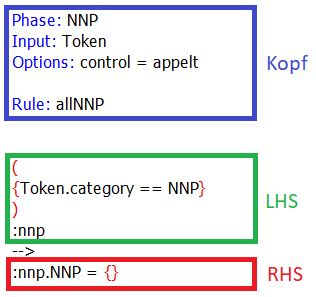
\includegraphics[scale=1]{Bilder/Regel-Bsp.png}
\caption{Beispielhafte JAPE-Regel [eigene Darstellung]}
\end{center}
\end{figure}

Im Kopf der Regel befinden sich die Parameter \textit{Phase}, \textit{Input}, \textit{Options} und \textit{Rule}.

 
\begin{enumerate}
\item Phase: Hier lässt sich eine Phase festlegen, in welcher die Regel ausgeführt werden soll. Dies kann wichtig sein, wenn z.B. eine Regel eine Annotation verwenden möchte, welche zuvor von einer anderen Regel angelegt werden muss. In unserem Projekt wurden für eine bessere Übersicht verschiedene Transducer angelegt, welche dann hintereinander durchlaufen werden. Daher wird die Phase im weiteren Verlauf der Arbeit nicht weiter verwendet oder behandelt.

\item Input: Das Definieren des Inputs ist vor allem später für die LHS von entscheidender Bedeutung. Hier wird angegeben, welche Annotationen in den regulären Ausdrücken abgefragt werden können.

Wenn ein Annotationstyp im Input nicht angegeben ist,jedoch in der LHS verwendet wird, führt dies zu einem Fehler beim Erstellen des Transducers. Wenn im Input Annotationen angegeben sind, welche in der LHS nicht verwendet werden, schadet dies unnötig der Laufzeit des Transducers.

\item Options: Hier können verschiedene Optionen zum verhalten der Regel in bestimmten Fällen angegeben werden. Dies beinhaltet hauptsächlich die Anpassung der \textit{control}-Option. Diese entscheidet über das Resultat der Regel, wenn sich etwa mehrere Annotationen der Ausgabe überschneiden. So kann etwa jede einzelne Annotation oder auch nur die längste Annotation (welche die kleineren abdeckt) ausgegeben werden. Andere Optionen wie \textit{negationGroupng} können benötigt werden, um bestimmte reguläre Ausdrücke in der LHS zu ermöglichen.

\item Rule: Hier wird der Name der Regel definiert. Dieser weist üblicherweise auf die Funktion der Regel, bzw. die erzeugte Annotation hin. Außerdem wird er oftmals als Feature der erzeugten Annotationen hinzugefügt, um die Nachvollziehbarkeit einer Verarbeitungslogik zu erhöhen. 
\end{enumerate}

In der JAPE-Regel befindet sich unterhalb des Kopfes die LHS.  Diese umfasst eine Menge von Regulären ausdrücken, basierend auf den Annotationen welche als Input deklariert wurden. Diese werden in dem Text gesucht und auf die angegebenen Bedingungen geprüft. Sollten gefundene Annotationen diese Erfüllen, so werden diese mit einem Label versehen. 

Ein Pfeil trennt die LHS von der RHS. Unterhalb der Pfeils befindet sich die RHS, in welcher abhängig von den vergebenen Labels nun neue Annotationen und deren Features mit Werten definiert werden können. 

Alternativ kann sich auf der RHS in einer JAPE-Regel auch JAVA-Code befinden um erweiterte Funktionalitäten nutzen zu können. Dies war für das Projekt jedoch nicht nötig, da die Ergebnisse der JAPE-Regeln ohnehin später in eine JAVA-Programm verwendet wurden. Daher wird diese Option im Verlauf der Arbeit nicht weiter berücksichtigt. \\ 

Der Aufbau von JAPE-Regeln soll an dem Beispiel in Abbildung X.X genauer erläutert werden:

Zunächst wird die Phase \textit{NNP} benannt und die \textit{Token}-Annotation als Input deklariert. Die \textit{control}-Option wird auf \textit{appelt} gesetzt. Diese wird im Normalfall verwendet und bewirkt, dass eine betroffene Stelle im Text nur von einer Regel genutzt werden kann\footnote{Setzen zwei Regeln am gleichen Startpunkt an, so erhält die Regel mit der längeren Übereinstimmung Vorrang, sind beide gleich lang, so erhält die Regel mit der höheren Priorität Vorrang, haben beide die gleiche Priorität, so erhält die Regel Vorrang, welche als erste in der Grammatik definiert wurde.\cite{tol09}}. Die Regel selbst wird mit \textit{allNNP} benannt, dies wird jedoch im Rest der Regel nicht wieder verwendet. 

In der LHS wird mit der Abfrage\\

$\{Token.category==NNP\}$\\

das \textit{category}-Feature der \textit{Token}-Annotation auf den Wert \textit{NNP} geprüft\footnote{Erinnerung: Die \textit{Token}-Annotation wird von dem Tokenizer erstellt, das \textit{category}-Feature und dessen Wert jedoch von dem POS-Tagger}. Die Abfrage entspricht also der Form\\

$\{Annotation.Feature==Wert\}$\\

Alle Tokens, welche diese Bedingung erfüllen, werden daraufhin mit dem Label \textit{nnp} versehen, welches auf die RHS der Regel übernommen wird. 

Unterhalb des Pfeils wird nun durch die Zeile\\

$:nnp.NNP=\{\}$\\

jede mit \textit{nnp} markierte Stelle mit der \textit{NNP}-Annotation versehen. In den geschweiften Klammern könnten dieser Annotation außerdem Features übergeben werden. Möchte man wie zuvor erwähnt den Namen der Regel als Feature hinzufügen, so lässt sich dies mit der folgenden Ergänzung tun:\\

$:nnp.NNP=\{rule=\grqq allNNP\grqq \}$\\

Damit ist eine neue Annotation Namens \textit{NNP} mit dem Feature \textit{rule} erzeugt, welche von späteren Regeln mit der einfachen Abfrage $\{NNP\}$ genutzt werden kann, ohne den Wert eines Features abfragen zu müssen.

\subsubsection{JAPE-Regeln in der Praxis}
In diesem Abschnitt werden einige der in der Sprachverarbeitung verwendeten JAPE-Regeln und deren Funktionsweise genauer erläutert. 

Ursprünglich war der Ansatz für die Erkennung von Systemnamen eine genaue grammatikalische Analyse zu nutzen um solche Namen komplett erfassen zu können. Dieser wurde jedoch nach verschiedene Tests für zu unpräzise befunden. Grund dafür war, dass in den Systemnamen keine ausreichende Regelmäßigkeit erkannt werden konnte, um ein verlässliche Erfassung zu gewährleisten. 

Daher wurde als nächstes ein Ansatz mit einer simpleren, jedoch auch besser umsetzbaren Methode verfolgt. Durch die Nutzung eines Gazetteers, kann die korrekte Erkennung von Eigennamen stark verbessert werden. Der einzige Nachteil ist, dass diese Eigennamen zuvor bekannt sein müssen, dies ist jedoch im betrieblichen Kontext gut umsetzbar. Um dies zu demonstrieren wurde ein ANNIE-Gazetteer mit einigen Systemnamen angelegt und sowohl für Beispiele, als auch für komplette Lastenhefte getestet. Daher wird im Folgenden anstelle einer JAPE-Regel der verwendete Gazetteer vorgestellt. Solch ein Gazetteer besteht aus einer Menge von \textit{.lst}-Dateien welche als Listen fungieren und mindestens einer \textit{.def}-Datei, welche definiert wie mit den einzelnen Listen umzugehen ist. In Abbildung X.X ist ein Ausschnitt einer solchen Listendatei zu sehen. Abbildung X.X zeigt die direkte Definition einer bestimmten Annotation innerhalb der Definitionsdatei. Dies ermöglicht das Einsparen einer JAPE-Regel, welche die standardisierte \textit{Lookup}-Annotation abfragen und einordnen muss.

\begin{figure}[H]
\begin{center}
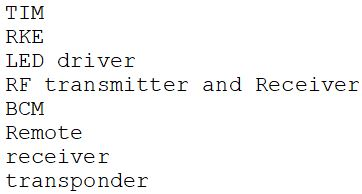
\includegraphics[scale=1]{Bilder/SystemNameGazetteer.jpg}
\caption{Ausschnitt der \textit{SystemName}-Liste des Annie-Gazetteers [eigene Darstellung]}
\end{center}
\end{figure}

\begin{figure}[H]
\begin{center}
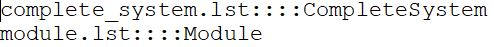
\includegraphics[scale=1]{Bilder/DefGazetteer.jpg}
\caption{Definitionsdatei des Annie-Gazetteers [eigene Darstellung]}
\end{center}
\end{figure}

Die Regel \textit{recognize\_conditional\_actor} wird dazu verwendet, im Falle einer Anforderung mit Bedingung den Akteur zu ermitteln, welcher durch die Bedingung eingeschränkt wird. Diese Anforderungen können dann später in die \textit{Boilerplate85} überführt werden, welche in Abschnitt X.X dargestellt ist. 

\begin{figure}[h!]
\begin{center}
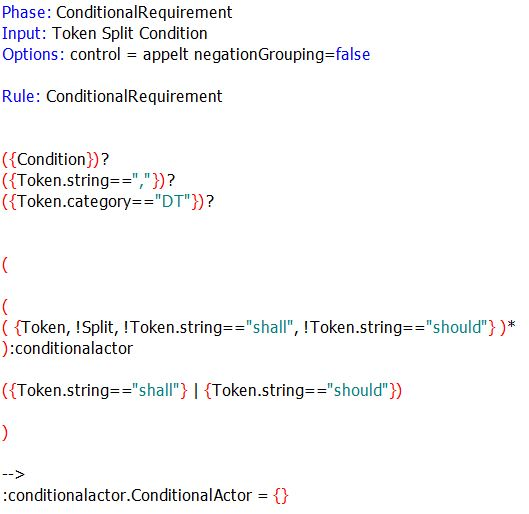
\includegraphics[scale=0.8]{Bilder/ConditionalActor.jpg}
\caption{JAPE-Regel zur Erkennung von eingeschränkten Akteuren [eigene Darstellung]}
\end{center}
\end{figure}

In der Phase und der Benennung der Regel sind soweit keine Besonderheiten. Als Input sind hier jedoch \textit{Token}, \textit{Split} und \textit{Condition}. Token ist die bereits bekannte Annotation des Tokenizers und Split ist eine Annotation des Sentence Splitters, welche das Ende einse Satzes (z.B. durch Punkt oder Leerzeile) markiert. Außerdem wird die eigens erstellte Condition-Annotation verwendet, welche auf Grundlage von Schlagwörtern wie \textit{if} oder \textit{when} die Bedingung in einem Satz erkennen und markieren kann\footnote{Auch zu dieser Annotation gibt es natürlich eine Regel, diese wird jedoch aus Platzgründen nicht genauer erläutert und befindet sich mit den restlichen Regeln in den Anlagen der Arbeit}. Außerdem wird die Option \textit{negationGrouping} auf \textit{false} gesetzt, um es zu ermöglichen mehrere negierte Abfragen auf der gleichen Token-Annotation auszuführen. \\

Generell muss die Regel die folgenden zwei Satzstellungen berücksichtigen können: 
\begin{enumerate}
\item Unter der Bedingung \textit{A}, soll das System \textit{B} die Aktion \textit{C} durchführen.
\item Das System \textit{B} soll die Aktion \textit{C} durchführen, unter der Bedingung \textit{A}.
\end{enumerate}
Die LHS der Regel beginnt daher mit einer optionalen Abfrage auf eine Condition, ein Komma und einen \textit{Determiner} (the, this, a usw.). Dies sorgt dafür, dass diese Elemente nicht mit als \textit{ContitionalActor} markiert werden, falls sie wie in \textit{1.} vor dem Akteur im Satz auftauchen. 

Daraufhin werden die folgenden Tokens als \textit{conditionalactor} getaggt, jedoch nur solange:
\begin{enumerate}
\item keine Split-Annotation enthalten ist,
\item kein \textit{shall}
\item und kein \textit{should} im Text auftauchen.
\end{enumerate}

Nachlaufend ist es jedoch nötig, dass eines dieser Wörter auftaucht (außerhalb des conditionaleactor-Taggings), da der Satz sonst nicht für die gewollte Boilerplate geeignet sein kann.

Damit ist LHS bzw. die Erkennung abgeschlossen und die als conditionalactor getaggten Bereiche werden mit der \textit{ConditionalActor}-Annotation versehen. Features werden dabei nicht benötigt. \\

Sobald alle benötigten Satzbestandteile erfasst sind, lässt sich auf deren Grundlage nun eine geeignete Boilerplate definieren. Diese wird mit der JAPE-Regel \textit{BP85\_bsp} in Abbildung X.X erkannt und markiert. 

\begin{figure}[h!]
\begin{center}
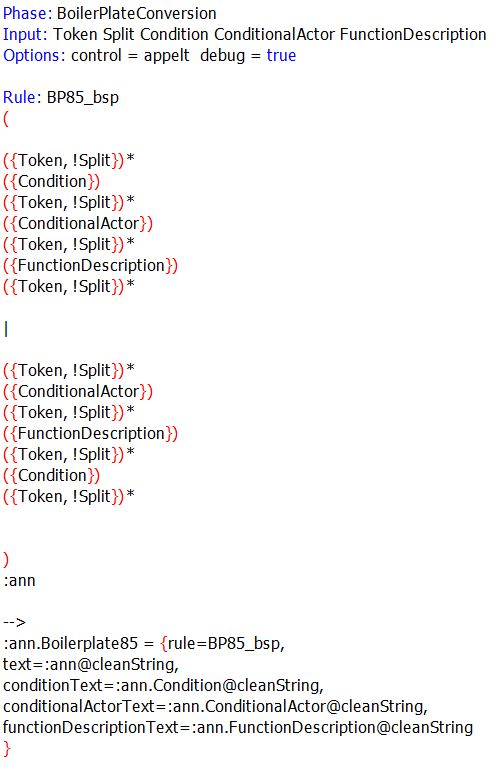
\includegraphics[scale=0.8]{Bilder/Boilerplate85Jape.jpg}
\caption{JAPE-Regel zur Markierung von Sätzen für Boilerplate85 [eigene Darstellung]}
\end{center}
\end{figure}

Im Regelkopf ist hierbei zu beachten, dass alle für die Boilterplate benötigten Satzbestandteile als Input definiert werden. In diesem Fall werden also die \textit{Condition}-, \textit{ConditionalActor}- und \textit{FunctionDescription}-Annotationen verwendet. 

Daraufhin werden in den regulären Ausdrücken der LHS die zwei Satzschemata abgefragt, welche schon bei der Erkennung des \textit{ConditionalActor} eine wichtige Rolle gespielt hatten:
\begin{enumerate}
\item Unter der Bedingung \textit{A}, soll das System \textit{B} die Aktion \textit{C} durchführen.
\item Das System \textit{B} soll die Aktion \textit{C} durchführen, unter der Bedingung \textit{A}.
\end{enumerate}

Zwischen den Satzbestandteilen vorkommende Tokens werden dabei ignoriert, solange diese keine \textit{Split}-Annotation enthalten, also mit Punkten oder Zeilenumbrüchen den Satz beenden. Alle Sätze die mit den Satzschemata entsprechen und die gestellten Bedingungen erfüllen werden als \textit{ann} gelabelt und auf der RHS der Regel verarbeitet.

Im Gegensatz zu den vorherigen Regeln ist auf dieser RHS die Vergabe von Features von entscheidender Bedeutung. Da man in dieser Regel verschiedene Annotationen zusammenfasst, ist es wichtig Informationsverlust zu verhindern, vor allem, weil die Satzbestandteile später noch vorliegen müssen um die Boilerplates zu befüllen. Daher erhält jede erstellte Boilerplate-Annotation auch ihren kompletten Text, sowie jeweils den Text jedes wichtigen Satzbestandteils als Feature. Dies macht es außerdem später im Programm einfacher diese abzufragen. Alle Features der Annotation sind in Abbildung X.X zu sehen. 

\begin{figure}[H]
\begin{center}
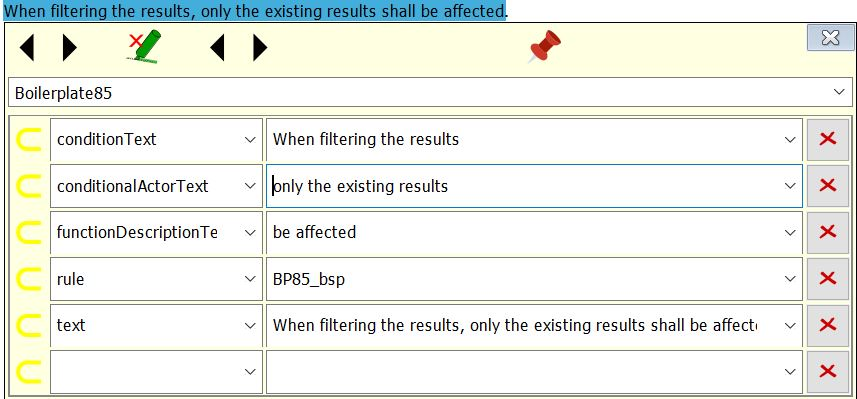
\includegraphics[scale=0.9]{Bilder/BP85Features.jpg}
\caption{Alle Features eines \textit{Boilerplate85}-Satzes in GATE [eigene Darstellung]}
\end{center}
\end{figure}

\subsubsection{JAPE Transducer in GATE}

Sobald alle benötigten JAPE-Regeln definiert sind, lassen sich diese unter JAPE-Hauptdateien zusammenfassen um die benötigte Anzahl von JAPE Transducern zu verringern. Es sollte jedoch nur soweit zusammengefasst werden, dass einzelne Transducer noch austauschbar sind, wenn man die Sprachverarbeitung ändern möchte. 
Die Transducer lassen sich (mit dem ANNIE-Plugin) über die Benutzeroberfläche von GATE leicht als Verarbeitungsressource anlegen und erhalten beim Initialisieren direkt die jeweilige JAPE-Datei. Syntaxfehler innerhalb der Dateien werden sofort erkannt und im Hauptfenster ausgegeben. 
Sollten keine Fehler vorhanden sein erhält man die fertige Verarbeitungsressource, welche man an beliebiger Stelle in die Verarbeitungs-Pipeline einbauen kann.
Obwohl in dem Programm GATE Embedded verwendet wurde und die Benutzeroberfläche somit nicht direkt verwendet werden konnte, bietet GATE die wichtige Funktion Corpora und Verarbeitungslogiken zu speichern und zu laden. Somit kann in man eine Verarbeitungslogik in GATE erstellen diese als sogenannte \textit{.gapp}-Datei speichern und anschließend in der Embedded-Version von GATE innerhalb des Programms laden. Außerdem lässt sich dabei der verwendete Corpus leicht ändern bzw. neu bestimmen. Das Laden einer solchen Datei in das Programm wird im folgenden Abschnitt genauer erläutert. 


\subsection{Converter-Funktionalität}
\subsection{GUI - Nutzerinteraktion und Workflow}
\section{mögliche Erweiterungen}
\section{Test}
\subsection{Methodik}
\subsection{Durchführung}
\subsection{Ergebnisse}
\chapter{Delta-Analyse}
\section{Architektur}
\section{Implementierung}
\section{mögliche Erweiterungen}
\section{Test}
\subsection{Methodik}
\subsection{Durchführung}
\subsection{Ergebnisse}
\chapter{Evaluation}
\subsection{Umsetzung der NLP-Architektur in unserem Werkzeug}
In diesem Abschnitt wird die Einordnung unseres Prototypen als NLP-Werkzeug in die von \cite{cop04} definierte Architektur behandelt. Die verschiedenen Schritte aus Kap. 2.2. haben wir bei der Analyse und Verarbeitung der Lastenhefte in Programmbestandteilen umgesetzt. Anhand der Verarbeitungskette unseres Werkzeugs können wir die prinzipiellen Aufgaben von NLP-Werkzeugen dort wie folgt einordnen:

\begin{enumerate}
\item \textit{Input Processing} - Einlesen von Quelldaten: Zunächst kann der Nutzer Dateien für die Verarbeitung im Programm eingeben. Dazu wählt der diese Dateien in der GUI des Programms aus. Unser Werkzeug extrahiert daraus dann den enthaltenen Text.

\item \textit{Morphologische Analyse} - Annotation der Worttypen: Mithilfe der Analyse des Textes durch die GATE-Verarbeitungslogik ANNIE werden einzelne Wörter aus dem Text auf ihre sprachliche Funktion hin überprüft. Dies ermöglicht die weitere Untersuchung bestimmter Worttypen, wie z.B. Nomen, nachdem diese gesammelt wurden. Nomen können etwa in JAPE-Regeln als \textit{NNP} abgefragt werden (siehe 4.x)

\item \textit{Part-of-Speech-Tagging} - Erkennung von Satzbausteinen: Für ein genaues Verständnis, worum es in einer Anforderung geht, müssen die einzelnen Bestandteile des Textes zugeordnet werden. In unserem Programm werden gefundene Wörter etwa dahingehend geprüft, ob diese ein System darstellen können, wenn sie zuvor als Nomen kategorisiert wurden. 

Auf dieser Basis können dann passende Boilerplates identifiziert werden. Für die spätere Befüllung der Boilerplates mit den korrekten Begriffen ist die korrekte Erkennung von Worten im Satzzusammenhang daher wesentlich.

\item \textit{Parsing} - Überführung in Boilerplates: Mithilfe des POS-Tagging wurden zuvor passende Boilerplates auf Basis gefundenen Annotationen innerhalb der Anforderung gefunden. Dies stellt nun die Grundlage für die Zusammensetzung der Boilerplates des entsprechenden Typs dar, indem Boilerplate-Objekte im Programm erzeugt werden. 

Die Platzhalter werden dann von den Begriffen aus der Anforderung ersetzt, womit schlussendlich eine Anforderung in der formalen Sprache der Boilerplates vorliegt.

\item{Disambiguation} - Zuordnung der richtigen Konvertierung: Im Parsing werden zunächst alle möglichen Konvertierungen auf Basis möglicher Boilerplate-Typen durchgeführt. Nach der Erzeugung der Boilerplates liegen somit möglicherweise verschiedene Möglichkeiten der Deutung vor, von denen einzelne unpräzise oder fehlerhaft sein können. 

Unpräzise Formulierungen können etwa durch eine hierarchische Anordnung der Boilerplates reduziert werden, wenn eine spezifische Boilerplate offensichtlich besser den Inhalt der Anforderung repräsentiert als eine eher allgemein formulierte. Die allgemeineren Boilerplates werden somit gleich ausgeschlossen, wenn eine bessere Konvertierung möglich ist. Siehe dazu auch Kap. 4.x.

Diese Unterschiede werden, sofern vorhanden, als mehrere Boilerplates im Programm dargestellt und an den Nutzer ausgegeben. Der Nutzer kann in der GUI dann die am besten zum ursprünglichen Anforderung passende Konvertierung auswählen.

\item \textit{Context Module} - Bewertung im Zusammenhang: Bei der Identifikation der best passendsten Boilerplate wurden in Kap. 4.x Vorschläge zur Abbildung der Semantik gemacht. Diese Ansätze ermöglichen dann die Automatisierung der Auflösung bestimmter Mehrdeutigkeiten, wenn diese das Verständnis des Kontextes aus dem Zusammenhang mehrerer Sätze erfordern. 

Im Kontext mehrerer Anforderungen kann der Nutzer im Rahmen des Review-Prozesses weitere Informationen über den Dokumentenkontext mit einfließen lassen. Dies kann etwa Informationen über vorige Anforderungen beinhalten, die bereits verarbeitet wurden, oder Meta-Informationen über das Anforderungsdokument wie etwa ergänzende, mitgeltende Unterlagen.

\item \textit{Text Planning} - Speichern der korrekten Boilerplate: Nach der Auswahl von einer richtigen Konvertierung innerhalb der GUI hat sich der Nutzer für eine Boilerplate entschieden, die in das Export-Dokument übertragen werden soll. Durch diese Festlegung wird im Programm die entsprechende Boilerplate in die OutputList der Konvertierung eingetragen.

\item \textit{Tactical Generation} - Erzeugung von Text aus BP-Objekten: Die Boilerplates liegen nach der Konvertierung zunächst als Objekte im Programm vor. Vor der Erzeugung des Ausgabe-Dokuments, das alle Anforderungen als Boilerplates enthält, müssen aus diesen Objekten der Text extrahiert werden. 

Dieser Text liegt in den einzelnen Objekten als Zeichenkette vor und wird mithilfe einer Methode formatiert. Im Programm wird bei der Dokumentenerzeugung der Text aller übernommenen Boilerplates abgefragt.

\item \textit{Morphological Generation} - Sprachliche Anpassung: In unserem ersten Entwurf der Prototypen wurde die Analyse auf englischen Text optimiert, da die Lastenhefte überlicherweise auf englisch verfasst sind (siehe Kap. 3.x). Die Boilerplates im Programm sind dementsprechend in englischer Sprache verfasst, wie auch das Ausgabe-Dokument.

Da der Text bereits innerhalb der Boilerplate-Objekte formatiert wurde bzw. vorliegt, entfällt hier eine aufwändige Anpassung an Sprache und ihre Grammatik.

\item \textit{Output-Processing} - Erzeugung des Anforderungsdokuments aus Boilerplates: Nachdem die einzelnen Zeichenketten aus den Boilerpaltes extrahiert wurden, liegen nun die einzelnen Anforderungen in formaler Sprache als Text vor. Die Anforderungen müssen nun vor dem Export in der richtigen Reihenfolge angeordnet und an das Layout des Dokumentes angepasst werden.

Der Nutzer wählt dazu eine Datei über die GUI aus, in welche die Anforderungen exportiert werden. Der Dateityp ist dabei prinzipiell unbeschränkt, zur Vereinfachung wurde sich jedoch auf reine Textdateien (.txt) beim Export beschränkt. 

Das Programm schreibt nun alle Anforderungen, getrennt durch Leerzeilen, in die Datei, sodass schlussendlich alle Anforderungen als Boilerplates exportiert sind.
\end{enumerate}

Der Arbeitsablauf des Programms lässt sich anhand des zustandswandlers in Abb. 4.x nachvollziehen. Dort ist die interne Verarbeitung unter Referenzierung der Stufen aus der NLP-Architektur als Prozess zwischen verschiedenen Akteuren dargestellt.
\section{Auswertung der Testresultate}
\section{Mehrwert?}
\section{Ziel erreicht? Hypothese reviewen und schwafeln}
\chapter{Fazit}
\section{Zusammenfassung}
\section{Ausblick}

\chapter{Notizen}
\begin{enumerate}
\item UML-Klassendiagramme im Vergleich zu Ontologien (Struktur, Beziehungen, Informatik-Bezug)
\item Nutzen von Ontologien, welcher Mehrwert kommt zur syntax durch sie hinzu?
\item Betriebliche Anforderungen an Tool: ACID aus DB? 
\item Aktivitätsdiagramm aus PA mit GUI-User-Interaktion, Konkretisierung dortiger Activities
\item Use-Case Diagramm beim Konzept, PA nur referenzieren
\end{enumerate}

\newpage
\begin{thebibliography}{20}
\bibitem[AWK06]{awk06} Christian Allmann, Lydia Winkler, Thorsten Kölzow. \glqq The requirements engineering gap in the OEM-supplier relationship.\grqq , Journal of Universal Knowledge Management 1.2 (2006): 103-111.
\bibitem[CA15]{ca15}Arora, Chetan, et al. \glqq Automated checking of conformance to requirements templates using natural language processing.\grqq{} IEEE transactions on Software Engineering 41.10 (2015): 944-968.
\bibitem[BAL10]{bal10}Helmut Balzert. \glqq Lehrbuch der softwaretechnik: Basiskonzepte und requirements engineering.\grqq , Springer-Verlag, 2010.
\bibitem[CAR52]{car52}Rudolf Carnap, \glqq  Meaning Postulates.\grqq{} , Philospohical Studies vol.3 S.65-73, 1952.
\bibitem[CHO57]{cho57} Noam Chomsky, \glqq  Syntactic Structures\grqq{} , Mouton \& Co., Feb. 1957.
\bibitem[COP04]{cop04}Ann Copestake, University Of Cambridge, \glqq Natural Language Processing\grqq , 2004.
\bibitem[DGE19]{dge19} Deutsche Gesellschaft für EMV-Technologie e.V. \glqq CRS Customer Requirements Specification\grqq, aus https://www.demvt.de/publish/viewfull.cfm?ObjectID=ba9a0878\_e081\\ \_515d\_74a3411df6771be8, abgerufen am 09.01.19.
\bibitem[FF11]{ff11} Farfeleder, Stefan, et al. \glqq DODT: Increasing requirements formalism using domain ontologies for improved embedded systems development. \grqq{} Design and Diagnostics of Electronic Circuits \& Systems (DDECS), 2011 IEEE 14th International Symposium on. IEEE, 2011.
\bibitem[FH14]{fh14} Fockel, Markus, and Jörg Holtmann. \glqq A requirements engineering methodology combining models and controlled natural language.\grqq{} Model-Driven Requirements Engineering Workshop (MoDRE), 2014 IEEE 4th International. IEEE, 2014.
\bibitem[HAO14]{hao14} Hao Wu, et al. \glqq  ILLINOISCLOUDNLP: Text Analytics Services in the Cloud.\grqq{}  LREC. 2014.
\bibitem[HE13]{he13} Alexander Heßeler, et al. \glqq Anforderungsmanagement: Formale Prozesse, Praxiserfahrungen, Einführungsstrategien und Toolauswahl.\grqq{} Springer-Verlag, 2013.
\bibitem[HE18]{he18} HELLA Geschäftsbericht des Geschäftsjahres 2017/2018, von https://www.hella.com/hella-com/assets/media\_global/2018.08.10\_HELLA\_Geschaeftsbericht\_2018\_geschuetzt.pdf, aufgerufen am 16.01.2019
\bibitem[HE19]{he19}Firma HELLA. \glqq Unternehmensinformationen in Kürze.\grqq , aus https://www.hella.com/hella-com/de/HELLA-im-Ueberblick-723.html, abgerufen am 09.01.19.
\bibitem[HL01]{hl01} Hubert F. Hofmann, Franz Lehner. \glqq Requirements engineering as a success factor in software projects.\grqq IEEE software 4 (2001): 58-66.
\bibitem[HP12]{hp12}Andrea Harant, Miriam Poethen. \glqq HOOD Capability Model für Requirements Definition und Requirements Management \grqq{} HOOD Ltd. 2012.
\bibitem[IR09]{ir09}BGH, \glqq Urteil vom 6. Juli 2000, I ZR 244/97\grqq Artikel beim Institut für Rechtsinformatik von der Universität des Saarlandes, 13. Oktober 2009
\bibitem[KN85]{kn85}Kapur, Deepak, and Paliath Narendran. \glqq  An equational approach to theorem proving in first-order predicate calculus.\grqq{}  ACM SIGSOFT Software Engineering Notes 10.4 (1985): 63-66
\bibitem[KR93]{kr93}Ryan, Kevin. \glqq The role of natural language in requirements engineering.\grqq{} Proceedings of the IEEE International Symposium on Requirements Engineering. IEEE, 1993.
\bibitem[LV10]{lv10}F. Langenscheidt, B. Venohr. \glqq Lexikon der deutschen Weltmarktführer: Die Königsklasse deutscher Unternehmen in Wort und Bild.\grqq ,  Deutsche Standards–Gabal Verlag Google Scholar (2010).
\bibitem[MW02]{mw02}Matthias Weber, Joachim Weisbrod. \glqq Requirements engineering in automotive development-experiences and challenges.\grqq , Requirements Engineering, 2002. Proceedings. IEEE Joint International Conference on. IEEE, 2002.
\bibitem[PR15]{pr15} Pohl, Klaus, Chris Rupp. \glqq Basiswissen Requirements Engineering: Aus-und Weiterbildung nach IREB-Standard zum Certified Professional for Requirements Engineering Foundation Level.\grqq{} dpunkt. verlag, 2015.
\bibitem[RS18]{rs18}Felix Ritter, Aaron Schul. \glqq Analyse aktueller NLP-Methoden und -Werkzeuge am Beispiel von GATE.\grqq{} Projektarbeit Fachhochschule Dortmund 2018, 18.11.2018
\bibitem[SB88]{sb88}Muggleton, Stephen, Wray Buntine. \glqq  Machine invention of first-order predicates by inverting resolution.\grqq{}  Machine Learning Proceedings 1988. 1988. 339-352
\bibitem[SHE07]{she07} L. Shen, G. Satta, A. K. Joshi. In Meeting of the Association for Computational Linguistics (ACL), \glqq  Guided learning for bidirectional sequence classification\grqq{} , 2007.
\bibitem[TOL09]{tol09}Dhaval Thakker, Taha Osman, Phil Lakin. \glqq Gate jape grammar tutorial.\grqq{} Nottingham Trent University, UK, Phil Lakin, UK, Version 1 (2009).
\bibitem[WE13]{we13} Weller, Katrin. \glqq Ontologien.\grqq{} (2013): 207-218.
\bibitem[ZG02]{zg02} Zowghi, Didar, and Vincenzo Gervasi. \glqq The Three Cs of requirements: consistency, completeness, and correctness.\grqq{} International Workshop on Requirements Engineering: Foundations for Software Quality, Essen, Germany: Essener Informatik Beitiage. 2002.
\bibitem[ZH17]{zh17} Zichler, Konstantin, Steffen Helke. \glqq Ontologiebasierte Abhängigkeitsanalyse im Projektlastenheft.\grqq{} Automotive-Safety \& Security 2017-Sicherheit und Zuverlässigkeit für automobile Informationstechnik (2017).



\end{thebibliography}
\end{document}
